\documentclass[]{sig-alternate-05-2015}
%\documentclass[12pt]{article}
%\usepackage{proceed2e}
%\usepackage[margin=1in]{geometry}
%\usepackage{setspace} % list packages between braces
%\onehalfspacing
\usepackage{times}
\usepackage{color}
\usepackage{amsmath}
%\usepackage[fleqn]{amsmath}
\usepackage{amsfonts}
%\usepackage{amsthm}
\usepackage{graphicx}
\usepackage{algorithm,algorithmic}
\usepackage{pgf}
\usepackage{tikz}
\usepackage{lipsum}
\usepackage{mathtools}
\usepackage{cuted}
\usetikzlibrary{arrows,automata}

%\documentclass[]{sig-alternate-05-2015}
%%\usepackage{proceed2e}
%\usepackage{times}
%\usepackage{color}
%\usepackage{amsmath}
%\usepackage{amsfonts}
%\usepackage{graphicx}
%\usepackage{algorithm,algorithmic}
%\usepackage{pgf}
%\usepackage{tikz}
%\usetikzlibrary{arrows,automata}


\newcommand*\xor{\mathbin{\oplus}}
\newtheorem{example}{Example}
\newtheorem{definition}{Definition}
\newtheorem{theorem}{Theorem}
\newtheorem{lemma}{Lemma}
\newtheorem{proposition}{Proposition}
\newcommand{\nd}[1]{{\color{red} nd: #1}} %comments made by naipeng
\newcommand{\df}[1]{{\color{blue} df: #1}} %comments made by Dileepa
\title{Model Checking Nash Equilibria in Probabilistic Games}
\author{Dileepa Fernando\\ Supervisor - A/P Jin Song Dong \\ School of Computing, \\ National University of Singapore.}
\begin{document}
\maketitle

\begin{abstract}
Verifying whether rational participants in a probabilistic distributed system would deviate from the specified behaviour is an important but challenging task. We term this problem as verifying nash-equilibria in probabilistic cooperative distributed multi-player games.
Existing algorithms only work for non-probabilistic systems. We develop a model checking algorithm for automatically verify nash-equilibria for probabilistic systems.
The algorithm is implemented based on a model checker - PAT (Process Analysis Toolkit). Using the algorithm and our tool, we performed a case study on analysing the first probabilistic secret sharing scheme. Algorithm was evaluated by applying to a continuous task sharing scenario.
\end{abstract}

% \begin{CCSXML}
%<ccs2012>
%<concept>
%<concept_id>10011007.10010940.10010992.10010998.10003791</concept_id>
%<concept_desc>Software and its engineering~Model checking</concept_desc>
%<concept_significance>500</concept_significance>
%</concept>
%<concept>
%<concept_id>10002950.10003648</concept_id>
%<concept_desc>Mathematics of computing~Probability and statistics</concept_desc>
%<concept_significance>300</concept_significance>
%</concept>
%<concept>
%<concept_id>10003752.10010070.10010099</concept_id>
%<concept_desc>Theory of computation~Algorithmic game theory and mechanism design</concept_desc>
%<concept_significance>300</concept_significance>
%</concept>
%<concept>
%<concept_id>10002978.10003014.10003015</concept_id>
%<concept_desc>Security and privacy~Security protoc4ols</concept_desc>
%<concept_significance>100</concept_significance>
%</concept>
%</ccs2012>
%\end{CCSXML}
%
%\ccsdesc[500]{Software and its engineering~Model checking}
%\ccsdesc[300]{Mathematics of computing~Probability and statistics}
%\ccsdesc[300]{Theory of computation~Algorithmic game theory and mechanism design}
%\ccsdesc[100]{Security and privacy~Security protocols}
%\printccsdesc
%
%\keywords{Model Checking; Nash Equilibria; Probabilistic Game; Contract Signing; Secret Sharing}
%\input{Introduction_new}
\section{INTRODUCTION}%need to be capitalized by UAI
% cooperative, concurrent, multi-player, probabilistic, finite state mechanism, perfect-inf,  

Many systems in the real-world involve collaboration of many distributed parties, e.g., Internet routing~\cite{SP04}, peer-to-peer file sharing~\cite{BCK10}, cooperative backup~\cite{LEB03}, etc. 
In many of such systems, participants may have conflict interests. Thus, it is natural to consider each party as rational, meaning that each party only collaborates if his benefit from collaborating is more than not collaborating. In this sense, the system is actually a game. 
An important property for such systems/games is to ensure that every rational player would not deviate from the expected behavior specified in the systems. That is to say, to pursue the most benefit, the rational players would all follow the system, i.e., the system is the nash-equilibrium in the concept of game theory -- no one derivate from the system because this would harm their benefits.

Traditionally, when designing a system, participants are assumed to be either ``good guys'' -- who follow  the system behavior, or ``bad guys'', who do everything in their power to break the system~\cite{AAH11}. Rational/selfish participants are seldom considered, and few systems\footnote{Notable exceptions include~\cite{AAH11,LCW06}} work correctly under the rational settings (as stated in~\cite{MMS08}). 

When the desired properties, such as security or reliability, of such systems are critical, whether every collaborator following the system becomes of great importance. In this case, precisely proving that the system is indeed the desired equilibrium is necessary. Such proofs are often manual, e.g., proofs in the contracting signing protocol~\cite{Rabin83} and the secret sharing protocol~\cite{HT04}. As the proof tasks are often heavy, manual proof is error-prone and inefficient, especially the designer of a system may not be an expert on formal proofs. Thus, automated proof is desirable. Model Checking\cite{BK08}, which is a precise way to verify systems and has many automated tool support, is a promising method.

Automated model checking tools for games exist, e.g., MOCHA~\cite{AHM98}, MCMAS~\cite{LQR09}, GAVS+~\cite{CKL11} and PRISM-games~\cite{CFK13}. The existing tools verify various types of properties in various types of games. However, none of them is able to verify the nash-equilibrium type of property -- whether following the system is the optimal strategy for each rational players, in concurrent games. Recently, an algorithm has been developed to verify such properties in a sub-class games which can be described using finite state mechanisms~\cite{MMS08}. However, this work only considered games without probability. In reality, many systems have probabilistic behaviours.
Some of the systems are inherently probabilistic. Economic and biology systems are examples. There are other systems that fail to achieve certain goals without involving probability, for example, it is proved that non-probabilistic secret sharing scheme is not practical in the rational settings~\cite{HT04}. Hence, we propose an approach to verify nash-equilibrium for probabilistic systems. 

\paragraph{Contributions.}
We develop a verification algorithm to verify whether a probabilistic game is a nash-equilibrium. 
We implement the algorithm based on PAT (Process Analysis Toolkit), which is a model checking platform providing efficient general probabilistic model checking algorithms~\cite{PAT}.
We perform a case study on analyzing a probabilistic secret sharing scheme~\cite{HT04}. The authors of the scheme first prove that no practical mechanism for secret sharing works without using probability in the rational setting and further provide the first secret sharing with the rational participants in mind. 
This case study first illustrates how our algorithm and tool help to ease the proofs of the non-existence of non-probabilistic scheme. Second, it shows how the tool automatically verifies the correctness of the probabilistic scheme. In addition, during verification, weaknesses of the probabilistic scheme have been found.
\section{RELATED WORK}

Nash-equilibria is a popular topic in game theory. Algorithms exist for finding nash-equilibria in games~\cite{FPT04, DMP07, Daskalakis13}. However, these works usually use simulation and mathematical analysis techniques~\cite{BFW06}. Model checking has the advantages of both simulation, being automatic, and mathematical analysis, covering all possible behaviors.
Hence, Model Checking has been applied to verify game theoretic properties, for example~\cite{Henzinger98, AM04, LR06}. Among these works, we highlight the following which focused on probabilistic behaviors and automatic model checking tools for games.

The model checker MOCHA~\cite{AHM98} has been widely used for verifying games, e.g.,~\cite{KR03, MS05, ZZPM12}. However, nash-equilibria checking is not explicitly supported, and probabilistic behaviours are not supported.
Recently, a tool PRALINE has been developed specifically for computing nash-equilibria~\cite{Brenguier13}, and a tool EAGLE is developed for verifying nash-equilibria for concurrent games~\cite{TGW15}. However, these tools do not support probability.

Model checker PRISM~\cite{KNP11} supports probabilistic behaviours, but does not explicitly support verifying game properties.
Using the Rubinstein's protocol as a case study, Ballarini et al. show that probabilistic model checking (using the model checker PRISM) can be used for game analysis~\cite{BFW06}. This work inspirits automated probabilistic model checking for games, but it is specific to the negotiation game (a bargaining between a buyer and a seller) framework and does not address nash-equilibria analysis.
Later, PRISM-Games extends the model checker PRISM to be able to verify turn-based games~\cite{CFK13}. PRISM-game is able to verify nash-equilibriums, but only for turn-based games.

Probabilistic model checking has been used to analyse multi agent dynamics \cite{hao2012probabilistic} . Two strategies to arrive at maximal dispersion outcome (MDO) \cite{hao2012probabilistic} in a generalized anti-coordination game has been discussed. Counter Abstraction is used to reduce the state space. MDO can be seen as some form of equilibrium of the multi agent game, but it is not the formal Nash Equilibrium. Hence, this work is an application of probabilistic model checking to a specific class of games and it does not generally address the concept of nash-equilibrium.  


%PRISM-Games~\cite{CFK13} and negotiation-games~\cite{BFW06} describes turn based games in abstract level and %application level respectively. They use CTL to define parametric game properties which are not limited to Nash-equilibrium. %Both works use PRISM model checker for verification.

%Negotiation games presents a case study on “Rubinstein’s protocol” which is a protocol defined for bargaining between a buyer %and a seller. Two pure strategies for the game are, accepting the most recent offer made by the opponent player or coming up %with a new offer. This case study analyses how mixing these strategies according to some probability distribution, result in %different expected utilities. Here model checking is used to derive the reaching probability of different offers according to a %predefined acceptance probability function. Negotiation game is a special form of a game where the strategy space is %continuous %hence cannot be formulated as a normal form game and as a result, Nash equilibrium cannot be found with %classical game theory %algorithms. They claim, using probabilistic model checking for this analysis as a novelty and their goal %is to extend this work to %the level of finding Nash equilibrium.
%
%Tajouddine et al.~\cite{TGV08} Improves the state space explosion in SPIN model checker by using abstractions for the %verification of game theoretic properties of auction protocols. This verifies the strategy-proof ness of “Vikrey auction” with a %novel abstraction technique. This abstraction is unique in the sense that it is defined based on the property to be verified.

The most relevant work is the one by Mari et al.~\cite{MMS08}. This work proposes a symbolic model checking algorithm for verifying nash-equilibrium in distributed cooperative systems. It is the first algorithm to automatically verify that it is in the best interest of each rational agent to follow exactly a given system~\cite{MMS08}. A player's all possible behaviour is modelled as a finite state mechanism. The given system describes which action should be taken in which situation (by honest/altruistic players), which is modelled as constrains on state transitions of a game tree. Infinite sequences of actions are tackled by using \emph{discount factor}~\cite{FT91} to decrease relevance of rewards that are far in the future, which allows them to only look at finite sequences of actions. The authors propose a notion of equilibrium which takes both \emph{Byzantine} players -- players that randomly take possible actions and ignore utilities/rewards, and a \emph{tolerance} of rewards -- the reward difference between following the system and deviating from the system, as parameters; and prove that using their algorithm the proposed equilibrium can be automatically verified by just looking at finite sequences of actions. This algorithm does not support verification of probabilistic systems. We adopt a similar specification framework of players and equilibrium, and develop nash-equilibria verification algorithm, which focuses on probabilistic systems. Even though we define the verification algorithms for distributed systems with cooperative actions, the algorithm can be easily extended to support distributed systems with turn based actions as well.

% discusses the importance of using model checking for finite concurrent systems. Classical game tree mechanisms usually fail in %this scenario due to large (possibly infinite) state spaces. Since the state space is finite, model checking techniques become %more useful in verifying game theoretic properties in these systems. This work verifies nash equilibriums with arbitrary errors %in distributed system protocols in the presence of byzantine nodes using a symbolic model checker called NuSMV. However, this %work does not handle probabilistic protocols.

%Rational cryptography is an emerging area which analyses cryptographic protocols. Main aim of these is to design security %protocols such that the best choice of a self-interested agent is to follow the protocol instead of violating it. Automated proofs in %rational cryptography is not trivial because it has a security proof as well as a game theoretic proof. Backes et al.~\cite{BCM13} %defines a Nash equilibrium verification tool (ProVerif) for automated verification of rational cryptographic protocols. Applied pi %calculus is used to model these rational cryptographic protocols. This is the first effort of automated verification of rational %cryptographic protocols. However, their verification is specific to rational file sharing protocol.\nd{the paper seems not published}
%
%Defining high level languages to model, classes of game theory problems has also been investigated. ‘rPATL’ is such a language %defined in 2013~\cite{CFK13}. This language is specifically designed to handle turn based stochastic games.

\section{BACKGROUND}
\subsection{Game Theory}
\label{subsec: game_theory}
Game theory is a wide area of research which is used in various areas such as economics, computer architecture,  computer security and robotics. Two main aspects of a scenario modelled in game theory are the well defined utility and the information, each player has \cite{OR94}. For a game theory problem, there has to be more than one party involved. 
\par In a broad sense, games theory categorizes four kinds of games namely strategic games, extensive games with perfect information, extensive games without perfect information and coaliational games.

\paragraph{Strategic Games}\cite{OR94}
In a strategic game we have a set $P$ of players and each player $P_i$ has a non empty set of actions $A_i$. Each $P_i$ has a preference relation $\geq_i$ defined in $A_1 \times A_2 \times \cdots A_n$ which denotes how a player is affected from different action combinations. An action is denoted $(a_1,a_2, \cdots , a_n)$. As a short notation to compact the action combination of the players other than $P_i$ we use $a_{-i}$. The action combination $(a_1,a_2, \cdots , a_n)$ can also written as $(a_{-i},a_i)$ when we want to explicitly differentiate between player $P_i$'s actions and actions of the other players. This notation can be extended to denote the action combinations of player sets. For a set $st$, $(a_{st},a_{[n]-st})$
denotes the corresponding actions are categorized w.r.t the player set. 
\newline A Pay off function is defined for a special case where the preference relation is a total order. 
\paragraph{Extensive games with perfect information}\cite{OR94}
These kind of games have a set $P$ of players and a set of sequences (finite or infinite) $H$ which stand for the history of actions of a game. A member $h \in H$ is called terminal (history towards end of a game) if $h$ is infinite or not a prefix of any other member in $H$. We use Z to denote the set of all terminal sequences in $H$. A preference relation (similar for strategic game) is defined for these terminal sequences. For all the non terminal sequences in $H$ a function $Turn: H \setminus Z \rightarrow P $  specifies the player who has the next move. A player can choose between a set of actions depending on his history $h$. Here perfect information refers to the fact that at any point of the game all the players have history information.

\paragraph{Extensive games without perfect information}\cite{OR94}
In contrast to extensive games with perfect information, this type of games have a probability distribution for the set of actions to perform given a history $h$. In addition to the probability, there are information partitions defined for each player. All the history sequences where the resulting action set is similar are categorized into same partition. When a player does not know his exact history but knows all the possibilities for history and his action set can short list the possible history values according to information partitions.

\paragraph{Coalitional games}

Coalitional games are described for the completeness. Coalition games have a set $P$ of players and it has a value function $V : \mathbb{P} P \setminus \phi \rightarrow \mathbb{R}$ to define the pay off value obtained for each coalition.

\paragraph{Nash Equilibrium}\cite{OR94}
Nash Equilibrium is a state of a game ending in which no player has a regret on the strategy he used when he cannot control the strategies of other players. We define a Nash equilibrium for a strategic game as follows. \newline

\begin{definition}
	For a  strategic game of player set $P$ and action set $A_1\times A_2 \times \cdots \times A_n$ and preference relation $\geq$ a nash equilibrium is defined as an action combination $a^{*} \in $ such that, \\
$	\forall P_i \in P$ \\
$(a_{-i}^{*},a_i^{*}) \geq_i (a_{-i}^{*},a_i) \forall a_i \in A_i$
\end{definition}
It is not always the case that, a nash equilibrium according to above definition exists. However, for any strategic game, a mixed strategy Nash equilibrium exists. Nash Equilibrium for other forms of games also have the same concept of best response. We will not discuss all the definitions here, and we will refer to specific Nash Equilibrium definitions in section \ref{sec: verification_algo}.

In computer science research, the most important aspect we look in game theory is, computation and verification of Nash equilibria. The computation complexity is highly dependant with the number of strategies. Calculating Nash equilibrium in strategic games is PPAD complete. \cite{DGP09},\cite{CD06}. \newline
Extensive form games are widely used to model actual games in real life where the players take turns. There are some applications that can be regarded as games and can be represented by non of the above game categories. For example, processes/protocols can be defined as finite state mechanisms. However, the closest representation of the above mentioned representations is extensive form. This representation itself is not very efficient. 

%\par
%Multiparty computation protocols can also be analyzed using game theory. \cite{ADGH06} and \cite{ADGH06} analyze how the Shamir secret sharing scheme can be modified to be resilient to coaliation attacks.
%In \cite{ADGH06} a general strategy for any player. The $m$ out of $n$ secret sharing is augmented with a mediator for the following game. Mediator has a random variable $c^t\in \{0,1\} $ for each time step such that $Pr(c^{t}=\alpha)$ and $h^{t}=fc^{t} + g^{t}$ if $c^{t}=1$ $h^{t}(0)=f(0)$ which is the value of the secret. otherwise $f(0)$ cannot be calculated since $g^{t}(0)$ would always be chosen to be $0$. If any player can calculate $h^{t}(0)$ at some iteration when $c^{t}=1$ then he would know the secret. The paper analyzes how the players can know the secret by acting as coaliators. They find an upper bound to $\alpha$ such that the game is $k$-resilient. Paper suggests some changes to the mediator's protocol such that expected running time is reduced.Can we verify k-resilience by using model checking?  We can verify k-resilience for specific $n$.Utility functions had to be defined to fit the conditions mentioned in the paper. 
%
%%%\includegraphics{strategy}
%
%\cite{CJM98} implements a natural deduction based model checker to identify attacks on security protocols. \cite{TL10} describes a PAT approach. This introduces a new language called "Seve" to specify security protocols and also introduces a translator to translate from "Seve" to RTS. to RTS.  
%
%Try model bitcoin.Look at contract signing.Do some review in PRISM papers.
%
%probabilistic trusted 3rd party.

\subsection{Model Checking}

It is essential to validate a software system against its requirement specification. For complex systems, these properties has to be verified before the system development. Requirements can be mathematically defined as properties while actual systems can be presented as mathematical models \cite{BK08}. Different system behaviours are referred to as models and the property verification procedure is called ``Model checking".
\newline
The properties to verify include deadlock freeness, starvation freeness, etc. Some systems may allow some degree of misfunctionality. By using model checking algorithms we can find/verify the error bounds, maximum error probability, etc. Properties can be categorized into safety properties and liveliness properties. NASA's deep space-$1$ space craft and validation of the execution engine of the core TM i$7$ processor\cite{KGNT09} are some of the successful usages of model checking.
\newline
The first step of model checking procedure is to specify the system model and the property to be verified in the language of model checking. Then simulations can be performed to have some confidence about the operation of the system model. Next step is to check whether the property is satisfied by the system. If the property does not hold then model checking tool can  generate a counter example. Based on the counter example, the system model can be refined iteratively until the property holds.
\newline
A major challenge of model checking is state space explosion in real time system models. Researchers in model checking have been working on reducing the state space by using various abstraction techniques such as binary decision diagrams\cite{MMS08} and partial order reduction\cite{alur1997partial}. These abstractions can be application specific or generic. Abstractions may also be property specific. 

Verifying game theoretic properties in protocols has become very important and tricky because, the original definitions of game representations and the generic algorithms to find the Nash equilibriums do not help a lot in optimizing protocol verification. As mentioned in the previous section, model checking research community strongly focuses on application and property specific optimizations. Developing model checking algorithms to verify game theoretic properties is very useful under this background. 
\newline
On the other hand, some real world protocols are easy to analyse when they are represented as games. Following section provides some examples of using model checking to verify game theoretic properties.
\newline

\section{APPLICATIONS OF MODEL CHECKING FOR GAME THEORY}

Contract signing protocols have game-like properties that can be verified by model checking. A two-party contract is an exchange agreement.Informally, if both parties perform the contract, they have some utility. If one party violates the contract, the violator gets more utility and the other party receives less. It is evident that designing a simultaneous contract signing protocol which is fair, without either a trusted third party or a partial commitment scheme is usually difficult in practice.\cite{Ben-Or1990} A simple example for a partial commitment scheme is as follows.

\begin{figure}[H]
	\centering
	\includegraphics[width=\textwidth]{non_zero_sum3}
	\caption{Exchange Example}
	\label{fig:contract_example}
\end{figure}

 Figure \ref{fig:contract_example} \cite{Buttyan1999} defines a protocol in which player $A$ sends a half coin before player $B$ provides the service. If player $B$ provides the service, player $A$ can send the other half of the coin. If player $B$ does not provides the service, player $A$ gets a negative reward, because he lost half a coin and he has another half of a coin which he can't use. If player $A$ does not send his first half of the coin, protocol does not proceed and both players have no loss nor gain. The utilities for $A$ and $B$ are shown within brackets. This is exactly an example for an extensive game with perfect information. A similar example about a certified email protocol is mentioned in \cite{Buttyan1999}. \newline
 Probabilistic protocols for contract signing introduces parameters quantify fairness. Rabin's protocol\cite{Rabin83} and BGMR protocol\cite{Ben-Or1990} are two such probabilistic contract signing protocols. Following are the major steps of Rabin's protocol.
 
 \begin{algorithm}[H]
 	\floatname{algorithm}{Protocol}  
 	\renewcommand{\thealgorithm}{}  
 	\caption{Rabin's Protocol}  
 	\label{protocol1}  
 	\begin{algorithmic}[1]
 		\STATE $\forall k$ Let $R(k)$ be a random number $\in \{1,2, \cdots ,N\}$
 		\STATE let $A$ , $B$ going to decide on contract $C$
 		\STATE Decide on dead line $D$
 		\FOR{$i= 1$ to $N$}
	 		\STATE $S=$ "I am committed to $C$ if $i=R(D)$" 
	 		\label{st: A_to_B}
	 		\STATE $M=sig_{A}(S)$ 
	 		\STATE $A \rightarrow_{M} B$
	 		\STATE $S=$ "I am committed to $C$ if $i=R(D)$"
	 		\label{st: B_to_A} 
	 		\STATE $M=sig_{B}(S)$ 
	 		\STATE $B \rightarrow_{M} A$ 
 		\ENDFOR
 		\STATE Generate $R(D)$
 	\end{algorithmic}
 \end{algorithm}
  if the players follow the protocol they both commit to the contract with a probability $1$. If we assume that authenticity of the messages are preserved, avoiding sending of the messages is the only way to cheat. There is a strategy with probability $\frac{1}{N}$ to make an honest player committed while a rational player is not committed \cite{Rabin83}. \newline
  BGMR\cite{Ben-Or1990} protocol does a slight modification to statements \ref{st: A_to_B} and \ref{st: B_to_A} by replacing the commitment probability which is increased over the iterations. Model checking can be used to verify and find cheating strategies in the above protocols \cite{Norman2006}. Usage of model checking occurs in these examples in the verification part.\newline
Formal definitions were introduced to specify fair-exchange/contract signing protocols as games. These definitions can be flexible to specify different fairness definitions and would be useful for formal verification \cite{Buttyan1999}. They define the concepts of fairness, safe fairness and Nash equilibrium fairness and how a fair-exchange game operates under imperfect information.\newline
  
  Modelling languages are defined to specify protocols as games \cite{KSRJ01} discusses about modeling non repudiation protocols as games (ATL) and verifies these protocols by using MOCHA.Proposed future work were verifying abuse free-ness in contract signing protocols and investigating strategy synthesis.

\section{MOTIVATION}
One research problem in game like protocols/systems is the need to find a most efficient representation for the analysis of game theoretic properties. Designing new modelling language constructs to automatically generate the game representation by the system model is highly essential.  Another research problem is finding verification and synthesis algorithms based on the representation. If proposed algorithms are time consuming, approximate algorithms can be introduced.\newline
We consider verifying the rationality of finite state concurrent systems. We restrict our analysis to extensive games with prefect information. To be more general, we would assume the system/protocol choices be probabilistic.
\section{SPECIFICATION}
\label{sec:mech} 
%Our analysis consider the parallel synchronous systems. This means that all the nodes/players in the system perform their state %transitions at once. Distributed systems which perform protocol steps collectively (not strictly synchronous) can also be %
%included in the above category. In this setting we have two kinds of players namely, Byzantine and Altruistic.

%A parallel synchronous system can be seen as a system which goes through state transitions. Each player performs a transition %to a local state based on his global state and the available actions from that global state.

As mentioned in the introduction, we consider distributed systems with multiple players who need to cooperate in order to achieve a goal. Games for such systems are inherently distributed with multi-players, rather than turn based. In addition, a system can be non-terminating, i.e., there are infinite executing steps for some players. For instance, a system (e.g., the case study protocol) can be executed unbounded number of times.

Games are often represented in a normal form -- a matrix of players, strategies and payoffs, or in an extensive form -- a finite game tree specifying the sequences of actions. Such specification is no longer suitable when the game has infinite execution steps. In order to model infinite games, we adopt the finite state mechanism representation defined in~\cite{MMS08} -- each player is specified as a finite state mechanism, potentially with loops. This allows us to specify infinite execution in a finite manner.

%In a game theory setting, actions of each player depends on the amount of information they have. Practically, a player may not %have full information about other player states and their actions.  But he should have sufficient information about the global %state to perform the state transition. This modeling and analysis happens in a third party point of view who can view all the %global information. We can draw a local finite state machine for each player to list out the possible actions and its local states. %However, this can be an under specification because, in some scenarios local state cannot decide whether it can perform an %action specified in the local finite state machine.

%\subsection{SPECIFICATION}

We use the formalism of finite state mechanisms~\cite{MMS08} to model all possible local states and local actions of players. All players' local states and actions together form all possible global states and actions in a game. 

Our contribution in this section is, extension of the finite state mechanism in \cite{MMS08} for probabilistic settings. We describe, how we changed the non-probabilistic representation to arrive at a probabilistic representation. First of all, we update the model of players to be probabilistic. Then we extend the state representation to be probabilistic. More importantly, we present the calculation of the value $v_i^{k}(Z, s)$ and worst value $u_i^{k}(Z, s)$ of a state in the probabilistic settings.

We start from general properties of players and end with specific properties of player types. 
Each player $i$ has a set of local states, denoted by $S_i$, a set of initial states, denoted by $I_i$, and a set of actions, denoted $A_i$.  Action set representation would follow from the definitions in section \ref{subsec: game_theory}.

Set of all the local actions can be denoted by $\hat{A} = \cup A_i$. Before defining the transition function we must define different player behaviours. We also introduce synchronized actions. The set of synchronised actions can be denoted by $A^s$. $A^s \subseteq \hat{A}$ 



\paragraph{Byzantine Player}
In a non-probabilistic setting, a Byzantine player is modelled as all possible local states and their corresponding feasible local actions.
In a probabilistic setting, a Byzantine player has exactly the same local states and the corresponding local actions, since probabilistic systems do not introduce additional local actions.
That is to say, similar as in the non-probabilistic setting, a Byzantine player can deviate from a system specification by performing actions that are not defined in the system.
In addition to perform extra actions, for the probabilistic actions in a system, a Byzantine player is able to deviate from the specification by changing the probability distributions of the actions. For example, if a system specifies a player's action as follows: the player toss a coin - with probability $1/2$ to be head and $1/2$ to be tail, if it is head, the player sends $1$, otherwise, sends $0$. A Byzantine player can deviate from the specification by changing the coin into a special one -- with probability $1/3$ to be head and probability $2/3$ to be tail. Furthermore, a Byzantine player is able to assign probability to non-probabilistic actions. For example, a system specifies a deterministic action of sending $1$, a non-probabilistic Byzantine player can deviate by sending $0$, a probabilistic Byzantine player can toss a coin -- with probability $\alpha$ to be head and probability $1-\alpha$ to be tail, and sends $1$ if it is head and sends $0$ if it is tail. To summarize, a Byzantine player is able to assign an arbitrary probability distribution (which adds up to $1$) to at a local state.



\paragraph{Altruistic Player}
An altruistic player follows system specification, and thus has predefined probability distribution for each probabilistic action. A probabilistic altruistic player covers the definition of non-probabilistic altruistic player as well. Each state has a unique probabilistic action defined. If only one action is defined it can be considered as a specific case of containing a single action of probability $1$.
%Locally, this can be modelled by adding the pre-defined probability to probabilistic actions and keeping other actions the same as in the non-probabilistic settings.

%Globally, in order to specify the hybrid actions, we need to distinguish which actions are probabilistic and which are not. Since the system specifies the distinction. At a global state, we are able to tell the probabilistic actions from the non-probabilistic actions.

Since local actions at a local states are feasible actions at the corresponding global states,

%this can be formally modelled by defining a function $P_i: S \times A_i \rightarrow \mathbb{R}$ where $\mathbb{R}$ ranges over $[0,1]$, with the requirement that
%at a global state $s$, \(\Sigma_{a \in A_i \wedge B_i(s,a)} P_i(s,a) = 1.\)

We model probabilities of performing local actions starting at given local states. Define $P_i: S_i \times A_i \rightarrow [0,1]$ , with the requirement that
$\forall s_i \in S_i$, \(\Sigma_{a_i \in A_i} P_i(s_i,a_i) = 1.\)

A local action $a_i$ is defined in local state $s_i$ $ \iff P_i(s_i,a_i) > 0$.

\paragraph{Rational Player}
A rational player is a special case of a Byzantine player who has the full power to change the probability distribution of actions at a state, driven by utility. We show that a rational player would always choose an action which gives the maximum utility with probability $1$.
Taking the simplest case with two actions,
\begin{itemize}
	\item If both of the actions lead to paths that give exactly the same utility, the probability distribution of the two actions does not influence the utility. Hence, we can assume the player choose one action with probability $1$, the other with probability $0$, without loss of generality.
	\item If the two actions lead to paths that give different utility, the player would choose the one gives bigger utility with probability $1$, the other with probability $0$.
\end{itemize}
The same reasoning holds for the case that the player has more than two feasible actions.
Therefore, we can safely model a rational player with non-probabilistic actions.


\paragraph{Local State Transition}
Function $B_i: S\times A_i\times S_i \rightarrow \mathbb{B}$ is used to specify the feasibility of player $i$ performing a action $a\in A_i$, which leads $i$'s local state to $s'\in S_i$, at a global state $s\in S$  -- if it is feasible, $B_i(s,a,s')$ is true, otherwise false.
The function $B_i$ is required to have two properties: \emph{serial} and \emph{deterministic}:
\begin{itemize}
	\item
	Serial property says that there is at least one action defined for each player at each global state, i.e.
	($\forall s \in S$, $\exists a \in A_i , \exists s' \in S_i$ s.t. $B_i(s,a,s')$ is true);
	\item
	The deterministic property says that a player's action $a$ should lead to a unique resulting local state, i.e. ($(B_i(s,a,s_1)=true \wedge B_i(s,a,s_2 )=true) \implies s_1 =s_2$.)
\end{itemize}
Due to the deterministic property,  we simply write $B_i(s,a)$ to represent that action $a$ is valid in a global state $s$, since the local state $s'$ is uniquely defined. Similarly, the global possible actions of all players are $B = B_1\times B_2\times\cdots\times B_n$.

%Using the above definitions, a  player's is defined as as a tuple $\langle S_i, I_i, A_i, B_i\rangle$. All players together actually form a game which is formally defined as the tuple $\langle S, I, A, B\rangle$. Note that adding probabilistic behavior does not change the actions and the states. Hence, we adopt this formalism and extend each action with a probability, see Section~\ref{ssec:prob}.

In non-probabilistic settings as well as probabilistic settings,
$\langle S_i, I_i, A_i, B_i\rangle$ defines a Byzantine player, since a Byzantine player can perform all actions that are feasible at a state, ignoring utility/rewards.
%Byzantine players can be used to model the ``bad guys", for example, the Dolev-Yao attackers for security protocols.
%
Recall that a system specifies which action should be performed at which state by which player, i.e., a system is a specification of altruistic players.
Similar to $B_i$, function $T_i : S \times A_i \rightarrow \mathbb{B}$ is defined to specify a player $i$'s behaviour of genuinely following the system -- $T_i (s, a)=true$ ($s\in S$, $a\in A_i$) if $i$ shall perform $a$ at state $s$ according to the system.
Since following the system (altruistic player) is always part of the possible behaviour, we have $T_i (s,a) \implies B_i (s,a)$. In addition, we assume the system does not have unspecified situation or deadlocks. Formally, we require that $T_i$ is non-blocking (i.e. $\forall s \in S,  \exists a \in A_i$, s.t. $T_i(s,a)$).
A system specifies the altruistic players, formally specified as $T=\langle T_1, \cdots, T_n\rangle$.%Note that there can be multiple valid actions at a global state.

Since that function $T_i$ models the altruistic player's behaviour, and $B_i$ models a Byzantine player's behaviour, given a set of  Byzantine players (denoted as $Z$) among the total $n$ players, the behaviour of Byzantine and altruistic players is summarised as:

\begin{equation*}
BT_i(Z,s,a_i,s'_i)=
\begin{cases}
B_i(s,a_i,s'_i) &  i \in Z \\
B_i(s,a_i,s'_i) \wedge T_i(s,a_i) & i \notin Z
\end{cases}	
\end{equation*}

\paragraph{Payoff Function}\cite{MMS08}

Player $i$'s payoff is defined as a function $h^{\psi}_i: S_i \times A_i \rightarrow \mathbb{R}$, i.e., for each global state transition and a global action, there is a payoff value for player $i$, denoted as numbers in $\mathbb{R}$. Here, ${\psi}$ is a set of global constraints. 
%The issue is that, each global state and global action pair
%may not have a payoff defined because some actions can be attributed to states which they have no connection with.
%   \cite{MMS08}Even though hi is defined for all the (global state, global action) pairs, in our setting, only useful information %would be given by the hi values defined for valid state transitions. Practically it may also not be meaningful to define pay-off %values for invalid state transitions.
Hence, $h = \langle h_1,\cdots,h_n\rangle$ denotes the payoff of all the $n$ players at any state for performing any action.
The payoff function can be directly adopted to the probabilistic settings since it is not influenced by adding probability.

\paragraph{Discount factor}
Let $\beta_i \in (0,1)$ is the discount factor for player $i$. The discount factor is used to decrease the relevance of rewards decreases in the future, so that to ensure efficient computation of a finite strategy in the settings of infinite games. We adopt the discount factor as well in order to handle infinite games in probabilistic settings.

\paragraph{Local Finite State Machine}
The local finite state machine for player $i$, in a probabilistic setting can be defined as $(S_i, I_i, A_i, BT_i, h_i, P_i )$

We can see how the local state machines can be combined to come up with the global state machine. 
$(S, I, A, h) =(\Pi_i S_i, \Pi_i I_i, \Pi_i A_i, \Pi_i h_i)$. 

The remaining components are $P_i$ and $BT_i$. \newline

We can define probabilities of global actions given a global state.
Global state $s \in S$ can be written as a local state sequence, $\langle s_1,s_2, \dots s_n \rangle$ and global action $a \in A$ can be written as local action sequence $\langle a_1,a_2, \dots a_n  \rangle$ as defined above. 
Now we can define, Probability function for global actions $P : S \times A \times \mathbb{P}([n]) \rightarrow [0,1]$. \newline

\begin{equation*}
P(s,a,Z)=
\prod_{i \notin Z} P_i(s_i,a_i)
\end{equation*}  

The global transition function $BT$ also should be updated to support synchronized actions.
We define set $J_i$ ,for $i \in 1 \dots n $  to count the number of occurrences of synchronized local action $a_i$ in the action sequence $a$.
\newline
$J_i$ = $\{k$  $ \vline$ $ k \in 1 \dots n \wedge a_i \in A^s \wedge a_i = a_k \}$. \newline

\begin{equation*}
BT(Z,s,a,s')=
\begin{cases}
\wedge _ i BT_i(Z,s,a_i,s'_i) &  \forall \text{ } i \text{, } a_i \notin A^s \\
\wedge _ i BT_i(Z,s,a_i,s'_i) \wedge (J_i(a) != 1 )  & otherwise
\end{cases}	
\end{equation*}


It should be noted that if $BT(Z,s,a,s')=false$ then  $s'$ is a deadlock state. Now, summarized global finite state graph in the probabilistic setting is defined by,
$(S, I, A, BT, h, P )$.

We can move on to value calculations on the global finite state graph. We would need two concepts called path and strategy.

\paragraph{Path}
With the above definitions, a non-probabilistic game can be specified as $(S,I,A,B,T,h,\beta)$. Given such a game with a set of Byzantine $Z$,
a path is defined as a sequence of possible $(s,a)$ pairs where $s \in S$ and $a \in A$. We denote a path as $X=\langle X_0, \cdots, X_n, \cdots\rangle$, where each step $X_t$ ($t\geq 0$) is a $(s,a)$ pair. We use $X_t^{(s)}$ to denote the first element of a step in a path -- the state $s$ and $X_t^{(a)}$ to denote the second element -- the action $a$. Path length is the number of global actions contained by the path.
A path $X$ is valid if $\forall t < |X| $, $BT(Z,X_t^{(s)},X_t^{(a)},X_{t+1}^{(s)})$ is true, meaning that the the transition from one step to the next step is valid.
% where $s_i(t)$ and $a_i(t)$ are the local state and local action at step $t$ in a path respectively.
%Extra notation can be introduced to extract local states and actions from global states and actions.

In non-probabilistic setting, the utility of a player $i$ in a path is evaluated by adding up the discounted payoff values along the path, formally,
$V_i(X)= \Sigma_{t=0}^{|X|-1}{\beta_i^{t} h_i(X_t^{(s)},X_t^{(a)})}$, where $|X|$ is the path length, which can be infinite. When the path length is infinite, $V_i(X)$ converges to an upper bound, because of $\beta_i$.

$Path_k(s,Z)= \{\pi | \pi \text{ is a path in }(M,Z) \wedge |\pi|=k\text{ and }\pi^{(s)}(0)=s \}$
%$Path_k(s,Z)= \{X | X$ is a path in $(\mathcal{M},\mathcal{Z})$ and $|X| = k$ and $X_0^{s} = s\} $
%This set defines the paths of length $k$ which starts from state $s$.
%These paths can be filtered by the maximum cardinality of the set of Byzantine agent that is allowed.
%$Path_k(s,f) = \cup_{|Z|\leq f}$ $Path_{k}(s,Z)$. When the path has infinite length, we can omit the subscript $k$.
In a probabilistic setting, a path denotes a set of paths that are reachable through unique probabilistic strategies of Altruistic players and a strategy of Byzantine players. A path tree can be denoted by $\{\pi\}$. A path tree of length $k$ is denoted by $\{\pi|_k\}$
The concept of a probabilistic path can be defined through the concept of probabilistic action. Each non deterministic action choice by the set of Byzantine players correspond to one path tree in the global graph.

\paragraph{Strategy}

To reason on a game, it is often needed to distinguish one player's actions from other players. Hence, the notion of strategy is defined as follows: A strategy of a player is a sequence of local actions of the player. A strategy at a state $s$ defines what a player would behave in the future. Depending on other players' actions, there will be multiple paths with multiple utility values. The minimum utility value is called the \emph{guaranteed outcome} of the strategy for the player at the state $s$. In the algorithm in~\cite{MMS08}, two important values are calculated: 
\begin{itemize}
	\item the \emph{value} of a state $s$ at horizon $k$ for player $i$ with Byzantine players $Z$, denoted as $v_i^{k}(Z, s)$, is defined as the guaranteed outcome of the best strategy of length $k$ starting ate state $s$;
	\item the \emph{worst case value} of a state $s$ ate horizon $k$ for player $i$ with Byzantine players $Z$, denoted as $u_i^{k}(Z, s)$, is defined as the guaranteed outcome of the worst strategy of length $k$ starting at state $s$.
\end{itemize}
In a probabilistic setting, a strategy is defined the same as in the previous section. The only difference is that all the strategies of an Altruistic player are assigned a probability. Strategies also appear as sets. $\forall path set \{\pi \}$
there is a corresponding strategy set $\{\sigma \}$ for player $i$. 

In addition to the state machine representation, we would add two definitions for global probabilistic action and a global probabilistic state.

\paragraph{States}
We extend the global state representation in~\cite{MMS08} with probability. We can consider resulting states of a probabilistic action as a single probabilistic state.

\paragraph{Actions}
Since some players are probabilistic, a global action is defined as a set of atomic actions where each action can be assigned a probability. 

Let $a \in A,$ $a_Z$ be the local action components of Byzantine players and $a_{[n]-Z}$ be the local action components of altruistic players. A probabilistic global action can be defined as, \newline

$ GA=\{ a \in A | \forall a',a'' \in GA, a'_Z = a''_Z  \wedge \cup_{b \in GA} b_{[n]-Z}=A_{[n]-Z} \wedge  \forall c',c'' \in GA, c'_{[n]-Z} = c''_{[n]-z} \implies c'=c'' \}$


An example action is presented in figure \ref{fig: prob_act}. Let $s= \langle s_1,s_2,s_3 \rangle \in S$. Let there are $3$ players $1,2,3$ with enabled action sets $\{a_1,a_2\}$, $\{b_1,b_2\}$ and $P\{c_1,c_2\}$ respectively. Let $1$ be an altruistic player. \\
$P_1(s_1,a_1)=p_1; P_1(s_1,a_2)=p_2;$

\begin{figure}
	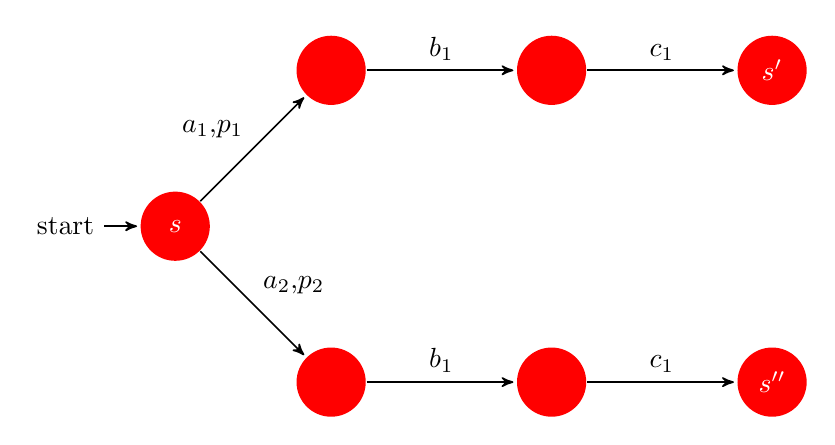
\begin{tikzpicture}[->,>=stealth',shorten >=1pt,auto,node distance=2.8cm,
	semithick]
	\tikzstyle{every state}=[fill=red,draw=none,text=white]
	\node[initial,state] (A)                    {$s$};
	\node[state]         (B) [above right of=A] {};
	\node[state]         (C) [below right of=A] {};
	\node[state]         (D) [right of=B] {};
	\node[state]         (E) [right of=C] {};
	\node[state]         (F) [right of=D] {$s'$};
	\node[state]         (G) [right of=E] {$s''$};
	
	\path (A) edge              node {$a_1$,$p_1$} (B)
	edge              node {$a_2$,$p_2$} (C);
	\path (B) edge              node {$b_1$} (D);
	\path (C) edge              node {$b_1$} (E);
	\path (D) edge              node {$c_1$} (F);
	\path (E) edge              node {$c_1$} (G);
	\end{tikzpicture}
	\caption{Probabilistic Global Action Example}
	\label{fig: prob_act}
\end{figure}
This probabilistic action can be written in set notation, $\{(a_1,b_1,c_1),(a_2,b_1,c_1)\}$. The other possible probabilistic actions are, \\
$\{(a_1,b_1,c_2),(a_2,b_1,c_2)\}$, $\{(a_1,b_2,c_1),(a_2,b_2,c_1)\}$ and $\{(a_1,b_2,c_2),(a_2,b_2,c_2)\}$.
same strategy of rational players is applied to both probabilistic choices because of the parallel synchronous nature of the system. Rational players do not have information about the probabilistic choice made by the altruistic player.
%\subsection{Probability Extension}\label{ssec:prob_act}

We extend the above specification to be able to specify probabilistic systems. A probabilistic system specifies the probability of each action in the system. To be more general, we allow hybrid probabilistic systems, meaning that some actions of a player in the systems are probabilistic, some of the actions can be deterministic. We also introduce synchronized actions. The set of synchronised actions can be denoted by $A^s$. $A^s \subseteq \hat{A}$ 

First of all, we update the model of players. Then we extend the state representation to be probabilistic. More importantly, we present the calculation of the value $v_i^{k}(Z, s)$ and worst value $u_i^{k}(Z, s)$ of a state in the probabilistic settings.

\paragraph{Byzantine Player}
In a non-probabilistic setting, a Byzantine player is modeled as all possible local states and their corresponding feasible local actions.
In a probabilistic setting, a Byzantine player has exactly the same local states and the corresponding local actions, since probabilistic systems do not introduce additional local actions.
That is to say, similar as in the non-probabilistic setting, a Byzantine player can deviate from a system specification by performing actions that are not defined in the system.
In addition to perform extra actions, for the probabilistic actions in a system, a Byzantine player is able to deviate from the specification by changing the probability distributions of the actions. For example, if a system specifies a player's action as follows: the player toss a coin - with probability $1/2$ to be head and $1/2$ to be tail, if it is head, the player sends $1$, otherwise, sends $0$. A Byzantine player can deviate from the specification by changing the coin into a special one -- with probability $1/3$ to be head and probability $2/3$ to be tail. Furthermore, a Byzantine player is able to assign probability to non-probabilistic actions. For example, a system specifies a deterministic action of sending $1$, a non-probabilistic Byzantine player can deviate by sending $0$, a probabilistic Byzantine player can toss a coin -- with probability $\alpha$ to be head and probability $1-\alpha$ to be tail, and sends $1$ if it is head and sends $0$ if it is tail. To summarize, a Byzantine player is able to assign an arbitrary probability distribution (which adds up to $1$) to at a local state.



\paragraph{Altruistic Player}
An altruistic player follows system specification, and thus has predefined probability distribution for each probabilistic action. Each state has a unique probabilistic action defined. If only one action is defined it can be considered as a specific case of containing a single action of probability $1$.
%Locally, this can be modelled by adding the pre-defined probability to probabilistic actions and keeping other actions the same as in the non-probabilistic settings.

%Globally, in order to specify the hybrid actions, we need to distinguish which actions are probabilistic and which are not. Since the system specifies the distinction. At a global state, we are able to tell the probabilistic actions from the non-probabilistic actions.

Since local actions at a local states are feasible actions at the corresponding global states,

%this can be formally modelled by defining a function $P_i: S \times A_i \rightarrow \mathbb{R}$ where $\mathbb{R}$ ranges over $[0,1]$, with the requirement that
%at a global state $s$, \(\Sigma_{a \in A_i \wedge B_i(s,a)} P_i(s,a) = 1.\)

We model probabilities of performing local actions starting at given local states. Define $P_i: S_i \times A_i \rightarrow [0,1]$ , with the requirement that
$\forall s_i \in S_i$, \(\Sigma_{a_i \in A_i} P_i(s_i,a_i) = 1.\)

A local action $a_i$ is defined in local state $s_i$ $ \iff P_i(s_i,a_i) > 0$.


We can also define probabilities of global actions given a global state.
Remember that a global state $s \in S$ can be written as a local state sequence, $\langle s_1,s_2, \dots s_n \rangle$ and global state $a \in A$ can be written as local action sequence $\langle a_1,a_2, \dots a_n  \rangle$. 
Now we can define, Probability function for global actions $P : S \times A \times \mathbb{P}([n]) \rightarrow [0,1]$. \newline

\begin{equation*}
P(s,a,Z)=
\prod_{i \notin Z} P_i(s_i,a_i)
\end{equation*}  

The global transition function $BT$ also should be updated to support synchronized actions.
We define set $J_i$ ,for $i \in 1 \dots n $  to count the number of occurrences of synchronized local action $a_i$ in the action sequence $a$.
\newline
$J_i$ = $\{k$  $ \vline$ $ k \in 1 \dots n \wedge a_i \in A^s \wedge a_i = a_k \}$. \newline

\begin{equation*}
BT(Z,s,a,s')=
\begin{cases}
\wedge _ i BT_i(Z,s,a_i,s'_i) &  \forall \text{ } i \text{, } a_i \notin A^s \\
\wedge _ i BT_i(Z,s,a_i,s'_i) \wedge (J_i(a) != 1 )  & otherwise
\end{cases}	
\end{equation*}


It should be noted that if $BT(Z,s,a,s')=false$ then  $s'$ is a deadlock state.

%Define $PA(s)=(PA_1(s),PA_2(s), \cdots ,PA_n(s))$.
%Let $P(s,a)=(P_1(s,a),P_2(s,a), \cdots ,P_n(s,a))$ For notational simplicity we would just use $P$.

%If the action is not probabilistic, it would be deterministic. \newline
%$ \forall s \in S$ and $a \in A , T_i(s,a)=T_i(s,b) \implies a=b$

%We define a probabilistic action player has full information about the local state he reaches when he performs the action. The probability distribution of the action components. The probability distribution of action components is provided by the protocol. We assume that, a Byzantine player has the full power of changing that probability distribution. In a probabilistic action, different action components may reach in different local states.
 %We do not have to consider the %resulting local state in the definition of $P_i$ due to the deterministic property.
%We require that at a global state $s$, $\Sigma_{a \in A_i \wedge B_i(s,a)} P_i(s,a) = 1$.
% $\Sigma_{a \in A_i \wedge B_i(s,a) \wedge P_i(s,a) \neq 1 } P_i(s,a) = 1$
%We don't allow $P_i$ value to be $0$ here in the analysis for the ease of explanation. If we allow $0$ we would have to reduce %the automata to cut down impossible action sequences.

%\paragraph{New Formalisms}
%In order to generalize these values to match probabilistic behaviour we define several new notations.

%$r$ refers to the definition in section of probabilistic actions.
%for each global action $a \in A^{r}(s)$ and player $i \in [n]$, \newline
%$\Theta (a,r,s,i) = \{y | y \in A_{-i}^{r}(s) \wedge r^{0}(y,s) = r^{0}(a_{-i},s) \wedge (y_j = a_j$  $ \forall j \in r^{0}(a_{-i},s)) \}$ . We can see that for given $r$ and $s$, the sets denoting $\Theta (a,r,s,i)$ forms a partition of $A^{r}(s)$ . Define this partition as $EP(r,s,i) = \{ \theta(a,r,s,i)| a \in A^{r}(s)$  and $i \in [n]\}$

%\paragraph{Actions}
% We would need to partition the set $A_i$ in to two namely, $A_i^{1}(s)$ and $A_i^{0}(s)$
%$ A_i^{1}(s) = \{ a \in A_i | P_i(s,a) \ne 1 \}$
%$ A_i^{0}(s) = \{ a \in A_i | P_i(s,a) = 1 \}$
%An action is a set of operations defined for a player in a particular global state $s$.
%We can define a set for atomic actions for a player $i$. $A_{at}(i)=\{a,b,c, \cdots\}.  $ $A_i(s) \subseteq A_{at}(i)$.
%$A_i(s)$ set can either be components of a probabilistic action or a non-deterministic choice at global state $s$.
%$A_i(s) = \{a |a \in A_{at(i)}  \wedge B_i(s,a)\}$
%This probability distribution is local to a player.
%$P_{(i,s)} : A_i(s) \rightarrow \Re^{+} $ and
%$\Sigma_{a \in A_i(s)} P_{(i,s)}(a) = 1$.


%Global probabilistic state is a set of global states $S_{pr} = \mathcal P (S_1 \times S_2 \times\cdots\times S_n)$ along with the probability of reachability under a strategy combination among the players. %A probabilistic state may contain only one global state with probability $1$. %A probabilistic state is a set of states that are reachable as a result of a valid global action sequence.\newline
%For any global probabilistic state $s_{pr} \in S_{pr}$ there is a probability distribution. $P_s : S_{pr} \rightarrow \Re^{+}$.\newline

%$\Sigma_{k \in S_{pr}} P_s(k) = 1$




\paragraph{Rational Player}
A rational player is a special case of a Byzantine player who has the full power to change the probability distribution of actions at a state, driven by utility. We show that a rational player would always choose an action which gives the maximum utility with probability $1$.
Taking the simplest case with two actions,
\begin{itemize}
\item If both of the actions lead to paths that give exactly the same utility, the probability distribution of the two actions does not influence the utility. Hence, we can assume the player choose one action with probability $1$, the other with probability $0$, without loss of generality.
\item If the two actions lead to paths that give different utility, the player would choose the one gives bigger utility with probability $1$, the other with probability $0$.
\end{itemize}
The same reasoning holds for the case that the player has more than two feasible actions.
Therefore, we can safely model a rational player with non-probabilistic actions.
%Note that this does not mean that probabilistic games are the same as non-probabilistic games, as we will show later in this section.
%So, all the actions of a rational player converge to non-deterministic choice.




%A local state set can be categorized into two sets named non-deterministic states and probabilistic states.
%Define,
%$nds_i : S_i \rightarrow B $ such that $nds_i(s)$ = true $\iff$ $s$ has a non-deterministic choice of local actions.
%
%We should also define a relation $par_i$. For any $b$ , $c$
%$\in S_i$, $b$ $par_i$ $c$ $\iff$ $\exists a \in A_i$, $s \in S$ s.t. $B_i(s,a,c)$=true and $b$=$s_i$.
%
%For any $s_i \in S_i$ we can define $parset_i(s_i) = \{ t| t \in S_i \wedge (t$ $par^{+} s_i )  \}$. This refers to the set of ancestors of $s_i$ along any feasible path.
%For any two global states $s=(s_1,s_2, \cdots ,s_n)$ and $t=(t_1,t_2, \cdots ,t_n)$ $\in S$, we can evaluate whether they are components of the same probabilistic state by traversing through the local parents of each local state component.
%$\forall i \in [1, \cdots ,n]$
%
%Probabilistic state can be denoted as, \newline
%$ s^{p} =\{(s,pr)| s \in S_1 \times S_2\times \cdots S_n,  \}$
\paragraph{States}
We extend the global state representation in~\cite{MMS08} with probability. Since a state may be reached via different paths. Each path that leads to the state may have different probability. In this case, we consider the global state with different probability two different states. In order to model it, we learn from the extensive form and use the history of states that lead to the current state to represent the current global state. 


\paragraph{Actions}
Since some players are probabilistic, a global action is defined as a set of atomic actions where each action can be assigned a probability. 

Let $a \in A,$ $a_Z$ be the local action components of Byzantine players and $a_{[n]-Z}$ be the local action components of altruistic players. A probabilistic global action can be defined as, \newline

$ GA=\{ a \in A | \forall a',a'' \in GA, a'_Z = a''_Z  \wedge \cup_{b \in GA} b_{[n]-Z}=A_{[n]-Z} \wedge  \forall c',c'' \in GA, c'_{[n]-Z} = c''_{[n]-z} \implies c'=c'' \}$
  
 
 An example action is presented in figure \ref{fig: prob_act}. Let $s= \langle s_1,s_2,s_3 \rangle \in S$. Let there are $3$ players $1,2,3$ with enabled action sets $\{a_1,a_2\}$, $\{b_1,b_2\}$ and $P\{c_1,c_2\}$ respectively. Let $1$ be an altruistic player. \\
 $P_1(s_1,a_1)=p_1; P_1(s_1,a_2)=p_2;$
 
 \begin{figure}
	 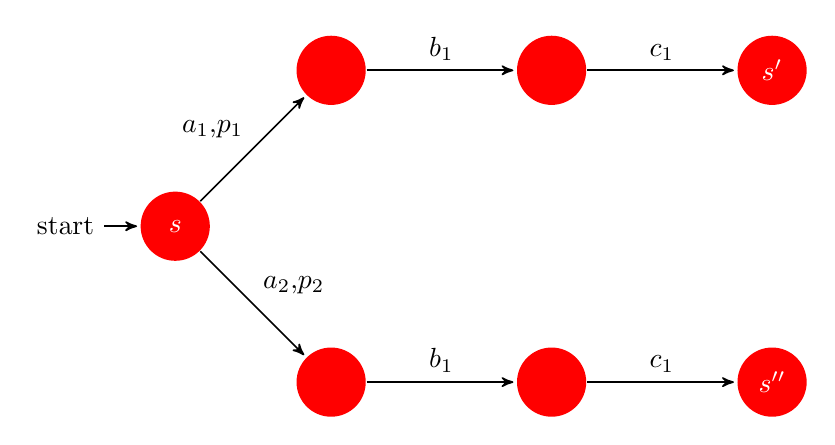
\begin{tikzpicture}[->,>=stealth',shorten >=1pt,auto,node distance=2.8cm,
	 semithick]
	 \tikzstyle{every state}=[fill=red,draw=none,text=white]
	 \node[initial,state] (A)                    {$s$};
	 \node[state]         (B) [above right of=A] {};
	 \node[state]         (C) [below right of=A] {};
	 \node[state]         (D) [right of=B] {};
	 \node[state]         (E) [right of=C] {};
	 \node[state]         (F) [right of=D] {$s'$};
	 \node[state]         (G) [right of=E] {$s''$};
	 
	 \path (A) edge              node {$a_1$,$p_1$} (B)
	 edge              node {$a_2$,$p_2$} (C);
	 \path (B) edge              node {$b_1$} (D);
	 \path (C) edge              node {$b_1$} (E);
	 \path (D) edge              node {$c_1$} (F);
	 \path (E) edge              node {$c_1$} (G);
	 \end{tikzpicture}
	 \caption{Probabilistic Global Action Example}
	 \label{fig: prob_act}
 \end{figure}
 This probabilistic action can be written in set notation, $\{(a_1,b_1,c_1),(a_2,b_1,c_1)\}$. The other possible probabilistic actions are, \\
  $\{(a_1,b_1,c_2),(a_2,b_1,c_2)\}$, $\{(a_1,b_2,c_1),(a_2,b_2,c_1)\}$ and $\{(a_1,b_2,c_2),(a_2,b_2,c_2)\}$.
 same strategy of rational players is applied to both probabilistic choices because of the parallel synchronous nature of the system. Rational players do not have information about the probabilistic choice made by the altruistic player.
\paragraph{Path}
In a probabilistic setting a path denotes a set of paths that are reachable through unique probabilistic strategies of Altruistic players and a strategy of Byzantine players. A path set can be denoted by $\{\pi\}$. A path set of length $k$ is denoted by $\{\pi|_k\}$
The concept of a probabilistic path can be defined through the concept of probabilistic action.

\paragraph{Strategy}

Strategy is defined the same as in the previous section. The only difference is that all the strategies of an Altruistic player are assigned a probability. Strategies also appear as sets. $\forall path set \{\pi \}$
there is a corresponding strategy set $\{\sigma \}$ for player $i$. 
%\paragraph{Reachability}
%Define a relation $nstate \subseteq S \times S$.
%Let $s$ , $s'$ $\in S$.
%$s$ nstate $s'$ $iff$ $ \exists a \in A$ s.t. $BT(Z,s,a,s')$.
%So, we can define the relation $reaches \subseteq S \times S$
%as $reaches $= $nstate^{+}$
%It should be noted that these relations are defined for notational convenience and would not add more information to the finite state mechanism.
%\paragraph{Probabilistic Value Function}
% $vp_{i}^{k+1}(Z,s)$ and $up_{i}^{k+1}(Z,s)$ are defined for probabilistic states where, $s \in S_i$


Hence, the probabilistic game is specified as $(S,I,A,B,T,h,P,\beta)$, where $P$ is newly added.



%Here, $A_i^{1}(s)$ has the components of the probabilistic strategy of player $i$ at global state $s$.Probabilistic strategy is itself %a non deterministic choice of a player. The set of non deterministic choices for a player at a given global state has an unknown %probability distribution. However, when choosing the path with minimal or maximal path value, the above unknown probability %distribution becomes $<0,0,$..$,1,0,0>$ where $1$ is for the action which directs to the maximal/minimal path accordingly.

%When given a global action we may need to filter out the players with probabilistic strategies and players who are not. First we %introduce an $n$-tuple of binary numbers where $1$ denotes a probabilistic strategy and $0$ denotes a non deterministic choice.

%$r \in \{0,1\}^{n}  = (r_1,r_2,$...$,r_n)$.
%We define two partitions $r^{0}(a,s)$ and $r^{1}(a,s)$.
%$r^{0}(a,s) =\{i | a_i \in A_i^{0}(s)  \} $
%$r^{1}(a,s) =\{i | a_i \in A_i^{1}(s)  \} $
%Define $A^{r}(s)$ as $\phi A_i^{r_i}(s)$


 We extend the following example in~\cite{MMS08} with probability, to show how a probabilistic system is modeled.
 \begin{example}\label{ssec:ex}
Suppose there are $m$ jobs $\{J_1, \cdots, J_m\}$, and $q$ tasks $\{T_0, \cdots, T_n\}$. Each job is consisted of a set of tasks.
A system, consisting of $n$ workers, specifies a sequence of tasks for each worker. A task sequence for player $i$ is denoted as $\mathcal{T}_i=\langle \tau(i,0), \cdots, \tau(i, l_i)\rangle$, where $l_{i}+1$ is the length of the sequence. When finishing one task, a work waits for the rewards. Once the rewards are received, the worker starts the next task. After finishing all tasks in the sequence (i.e., after finishing $\tau(i, l)$), a worker repeats the sequence of tasks from beginning (i.e., task $\tau(i,0)$). Once a job is completed, the rewards are granted to the works who finished the tasks that compose the job. Assume that tasks for different jobs do not overlap. In completing a job, if more than one workers finish the same task, all of them will be rewarded.
A worker may deviate from the system by delaying execution of a task or not executing a task in his task sequence.

We extend the above example system with probability. In addition to the task sequence, each worker is assigned a probability $0.4$ to take the next task, and probability $0.6$ to skip the next task. For example, a work will toss a coin before taking the next task: if it is head, he takes the next task, if it is tail, he skip the next task.
\end{example}

Similar to the formalization in~\cite{MMS08}, in the example, a worker's states are modelled as $X_i=Y_i\times Z_i$, where $Y_i$ is the worker's task sequence and $Z_i$ is the status of each task, $Z_i=\{0, 1, 2\}$, with $0$ denoting that the worker is not working, $1$ denoting that the work finishes his assigned work, and $2$ denoting that the current (finished) work is used by a job. Note that in this example, the states for altruistic, rational or Byzantine players/workers are exactly the same.
%
A player's initial state is $I_i=(\tau(i,0),0)$. Since the only deviation is not taking the task, the set of actions for all players are the same, i.e., $A_i=\{a^i_0, a^i_1\}$, where $a^i_0$
denotes the player $i$ does not take the task, and $a^i_1$ denotes that the player $i$ will take the task. The action $a_1$ will lead a state $(\tau(i, j), 0)$ to $(\tau(i, j), 1)$, and the action $a_0$ leads to a self-loop. The transition from $(\tau(i, j), 1)$ to $(\tau(i, j), 2)$ happens if the task $\tau(i, j)$ is used for a job. Note that it does not needs actions from players.
Hence, $S=\langle (Y_1, Z_1), \cdots, (Y_n, Z_n)\rangle$, $I=\langle(\tau(1,0), 0),\cdots,(\tau(n,0),0)\rangle$ and $A=\{\{a^1_0, a^1_1\}, \cdots, \{a^n_0, a^n_1\}\}$.

We use the function $\pi_i$ to project a global state $s$ or a global action $a$ to the local state of player $i$, and use $a^i_{\tau}$ to denote the empty action of player $i$. The function $B_i(s, a, s')$ is defined as follows:
\[
\begin{array}{l}
B_i(s, a_i, s')=\\
\ \left\{
\begin{array}{ll}
\mbox{true} &\mbox{if}\ \pi_i(s)=(\tau(i,j),0), \pi_i(s')=(\tau(i,j), 0), a_i=a^i_0\\
\mbox{true} & \mbox{if}\ \pi_i(s)=(\tau(i,j),0), \pi_i(s')=(\tau(i,j), 1),a_i=a^i_1\\
%\mbox{true} & \mbox{if}\ \pi_i(s)=(\tau(i,j),1), \pi_i(s')=(\tau(i,j), 2), a_i=a^i_{\tau}\\
%            & \tau(i,j)\ \mbox{is completed and needed for a job}\\
%\mbox{true} & \mbox{if}\ \pi_i(s)=(\tau(i,j),1), \pi_i(s')=(\tau(i,j), 1), a_i=a^i_{\tau}\\
%            &\tau(i,j)\ \mbox{is not completed or not needed for a job}\\
%\mbox{true} & \mbox{if}\ \pi_i(s)=(\tau(i,j),2), \pi_i(s')=(\tau(i,(j+1)\%l_i), 0), a_i=a^i_{\tau}\\
\mbox{false}& \mbox{otherwise}
\end{array}
\right.
\end{array}
\]
The first case says that if a player $i$'s next job is $j$, he can choose to not take the task ($a_i=a^i_0$), and this action leads to a state where $i$'s local state does not change ($\pi_i(s')=\pi_i(s)$). The second case models that if the player takes the task ($a_i=a^i_1$), the action leads to a state where the local state of $i$ changes into $\tau(i,j), 1)$.
%The third case represents that if the player's task is finished and is used for a job, then the status of his task is changed to $2$, otherwise, the status of the task remains to be $1$ (the fourth case). The fifth case states that if the task is rewarded, then the system automatically transit the state of the player to the beginning status of the next task. 

Differing from the definition in~\cite{MMS08}, the function $T_i(s,a_i)$ in this system is defined exactly the same as $B_i(s,a_i)$, since both of the actions $a^i_0$ and $a^i_1$ are enabled in the probabilistic system.
\begin{equation*}
T_i(s,a_i)=
\begin{cases}
\mbox{true} &\mbox{if}\ \pi_i(s)=(\tau(i,j),0), a_i=a^i_0\\
\mbox{true} & \mbox{if}\ \pi_i(s)=(\tau(i,j),0), a_i=a^i_1\\
\mbox{false} & \mbox{otherwise} 
\end{cases}
\end{equation*}
%\begin{figure}
%	\centering
%	\includegraphics[width=\columnwidth]{state_diagram_cropped}
%	\caption{State Diagram Example}
%	\label{fig:state_diagram_ex}
%\end{figure}
%For instance, assume there are $3$ workers, worker $W_1$, assigned job $J_1$, worker $W_2$ assigned job $J_2$, and %worker $W_3$ assigned job $J_1$. The task sequence of $W_1$ is $T_0,T_1,T_0,T_1,T_0,T_1 \cdots$, the task sequence of %$W_2$ is $T_1,T_0,T_1,T_0,T_1\cdots$. For each task, a worker has $3$ states, denoted by the value of $Z_i$: $z_i=0$ %means that the worker does not start working on the task; $z_i=1$ means that the worker is working on the task; and $z_i=2$ %means that the worker has completed the task. Let $Y_i= \{0,1\}$ where $0$ and $1$ denoting the position index in $\tau_i$. %State space for worker $i$ is $Y_i \times Z_i$. Let the initial local state of all the workers be $I=(0,0)$.

%The function $\gamma _i(s)$ denotes whether the current task is already completed at the global state $s$. This is sufficient to %show the involvement of the global state in the automata $B_i$. The function defines set of global states that are allowed to %arrive at the completed state at the presence of any input. ($a_i = 1$ or $a_i = 0$). The knowledge about global state is %considered to be transparent. Evaluation of the function will be discussed later. Now, we can define the pay-off function $h_i$.
The payoff function is defined the same as original as follows.
\begin{equation*}
\text{$h^{\psi}_i(s_i,a_i)=$}
\begin{cases}
\text{-1} &  \text{$\pi_i(s)=(\tau(i,j),0) \wedge (a_i = a^i_1) $} \\
\text{4} & \text{$\pi_i(s)=(\tau(i,j),2)$} \\
\text{0} & \text{otherwise}
\end{cases}	
\end{equation*}
The first case represents that the player works for a task, meaning that the player is paying, instead of gaining, and thus the payoff is negative. 
The second case capture the situation that the player's task is used in a job and thus the player is paid with positive payoff value. If the player does not work then he gains nothing and pays nothing, and thus has payoff value $0$. 

The probabilistic function $P_i(s, a_i)$ is defined for altruistic player as follows:
\begin{equation*}
P_i(s_i, a_i)=
\begin{cases}
%\left\{
%\begin{array}{ll}
%p& \mbox{if}\ i\in Z, a_i=a^i_0\\
%1-p &\mbox{if}\ i\in Z, a_i=a^i_1\\
%&\mbox{where}\ p\ \mbox{is any value between}\ 0\ \mbox{and}\ 1\\
%\end{array}
%\right.\\

\begin{array}{ll}
0.6& \mbox{if}\  a_i=a^i_0\\
0.4 &\mbox{if}\  a_i=a^i_1
\end{array}

\end{cases}
\end{equation*}
If a player is a Byzantine player $i\in Z$, then the probability can be an arbitrary distribution ($p$ can be any value between and include $0$ and $1$).
If a player is an altruistic player $i\not\in Z$, the probability distribution is pre-defined by the system ($0.6$ for not taking the task and $0.4$ for taking the task).

%Finally, all actions of a player are probabilistic, hence, $PA_i(s)$ is defined as follows:
%\begin{equation*}
%PA_i(s)=
%\begin{cases}
%\{a^i_0, a^i_1\} & \mbox{if}\ T_i(s,a_i)=\mbox{true}\\
%\emptyset & \mbox{otherwise}
%\end{cases}
%\end{equation*}
%$z_i=2$ only if a job is completed. In this case all the workers who took part to complete the tasks corresponding to the job %receive, a pay-off of $4$. First case corresponds to working on a non completed task where the worker receives a pay-off of %$-1$. Second case denotes the scenario of completing a job and in that situation, all the workers involved in the tasks %corresponding to the job, receive a utility of $4$ each.  $T_i$ in this mechanism is the same state machine without the %transitions corresponding to ($a_i = 0$).

%This mechanism can be easily extended to a probabilistic version by introducing $P(s,a)$. \newline
%$P(s,1)=0.4$ , $P(s,0)=0.6$.


 

 

\section{VERIFICATION ALGORITHM}
\label{sec: verification_algo}
We are going to verify the Nash Equilibrium of synchronous parallel finite state mechanisms. In order to define the equilibrium we should define a utility function with respect to the execution of the protocol. The concepts of $path$ and $strategy$ has to be used in order to define utility.


%We ca
%The above set outputs a set of global actions which has the exact same set of non deterministic local actions as $a$ and all the other local actions are probabilistic actions. The set enumerates on all the possible probabilistic local action by keeping the non deterministic local actions in $a$ constant. We can use this set to find the expected path values when the set of non deterministic actions is specified.

The dynamic programming algorithm to evaluate the value and the guaranteed outcome at horizon $k$ for player $i$ from a global state $s$ is as follows.


$v_{i}^{0}(Z,s) = u_{i}^{0}(Z,s) =0 $ \cite{MMS08} \newline

\begin{equation}
\begin{split}
v_{i}^{k+1}(Z,s)=
\begin{cases}
i \in Z &
\\max _{a_i \in A_i(s)}\{
min_{a_{Z-\{i\}} \in A_{Z-\{i\}}}\{
\\E_{a_{[n]-Z} \in A_{[n]-Z}(s)} (h_i(s,\langle a_{z-\{i\}},a_i,a_{[n]-Z} \rangle) +\\ \beta_i{v_i}^{k}(Z,s') | BT(Z,s,\langle a_{-i},a_i \rangle,s')  ) \} \}\\
i \notin Z &
\\E_{a_i \in A_i(s)}(min _{a_{Z} \in A_{Z}(s)}\{
\\E_{a_{[n]-Z-\{i\}} \in A_{a_{[n]-Z-\{i\}}}}( h_i(s,\langle a_{[n]-Z-\{i\}},a_{Z},a_i \rangle) +\\ \beta_i{v_i}^{k}(Z,s') | BT(Z,s,\langle a_{-i},a_i \rangle,s') )\} ) 
\end{cases}
\end{split}
\end{equation}

 
\begin{equation}
\begin{split}
u_{i}^{k+1}(Z,s)=
\begin{cases}
i \in Z &
\\min _{a_i \in A_i(s)} \{
min_{a_{Z-\{i\}} \in A_{Z-\{i\}}}\{
\\E_{a_{[n]-Z} \in A_{[n]-Z}(s)} (h_i(s,\langle a_{z-\{i\}},a_i,a_{[n]-Z} \rangle) +\\ \beta_i{u_i}^{k}(Z,s') | BT(Z,s,\langle a_{-i},a_i \rangle,s')  )\} \}\\
i \notin Z &
\\E_{a_i \in A_i(s)} (
min _{a_{Z} \in A_{Z}(s)}\{
 \\E_{a_{[n]-Z-\{i\}} \in A_{a_{[n]-Z-\{i\}}}} (h_i(s,\langle a_{[n]-Z-\{i\}},a_{Z},a_i \rangle) + \\ \beta_i{u_i}^{k}(Z,s') | BT(Z,s,\langle a_{-i},a_i \rangle,s')  )\} )
\end{cases}
\end{split}
\end{equation}

In the probabilistic setting, value functions for individual paths become value functions for  path tree from some state. $v_i(\{\pi\})$ and $v_i(\{\pi|k\})$ represent value of the player $i$ in path tree $\{\pi\}$ and the value of length $k$ horizon of path tree $\{\pi\}$  

%$\forall s_i \in S_i$, $ \exists s_{pr} \in S_{pr}$ s.t. $\forall t \in S_{pr} , t_i=s_i$

%Probabilistic state for $s_i \in S_i$ can be defined as, \newline
%
%$PS(s_i)=\{t | t \in S \wedge t_i=s_i \wedge \exists s_0 \in I , s0$ reaches $t \}$
%
%Now we can define the values of the game in terms of player $i$'s states.
%$vp_{i}^{k+1}(Z,s_i)= E_{x \in PS(s_i)}(v_{i}^{k+1}(Z,x))$ and $up_{i}^{k+1}(Z,s_i)=E_{x \in PS(s_i)}(u_{i}^{k+1}(Z,x))$

%\df{The above equation is finalized. Calculation of probability of reaching states is handled follows. Consistency of the symbols have to be checked }


%$v_{i}^{0}(Z,s) = u_{i}^{0}(Z,s) =0 $ \cite{MMS08} \newline
%$\forall a_i \in A_i $, \newline
%$v_{i}^{k+1}(Z,s,a_i) = min\{\Sigma_{r \in \{0,1\}^{n} } \Sigma_{\Theta \in EP(r,s,i)} \Sigma_{{a_{-i}} \in \Theta}$ $ \Pi_{q \neq i}$ $P(s,a_q)\{ h_i(s,<a_{-i},a_i>)  + \beta_iv_i^{k}(Z,s')  | BT(Z,s,<a_{-i},a_i>)\} \}$\newline
%$v_{i}^{k+1}(Z,s)=$\newline
%$max \{ \Sigma_{a_i \in A_i^{1}(s)} v_{i}^{k+1}(Z,s,a_i),$\newline
%$ max _{a_i \in A_i^{0}(s)}\{v_{i}^{k+1}(Z,s,a_i) \} \}$\newline
%
%$u_{i}^{k+1}(Z,s,a_i) = min\{\Sigma_{r \in \{0,1\}^{n} } \Sigma_{\Theta \in EP(r,s,i)} \Sigma_{{a_{-i}} \in \Theta}$ $ \Pi_{q \neq i}$ $P(s,a_q)\{ h_i(s,<a_{-i},a_i>)  + \beta_iu_i^{k}(Z,s')  | BT(Z,s,<a_{-i},a_i>)\} \}$\newline
%$u_{i}^{k+1}(Z,s)=$\newline
%$min \{ \Sigma_{a_i \in A_i^{1}(s)} u_{i}^{k+1}(Z,s,a_i),$\newline
%$ min _{a_i \in A_i^{0}(s)}\{u_{i}^{k+1}(Z,s,a_i) \} \}$



To determine $v^{k}_i(Z,s)$ at a global state $s$, we should consider all the globally valid local actions for player $i$. For each of these actions, Byzantine players can choose a combination of actions which minimize the expected pay-off for player $i$. Player $i$ can calculate the maxi-min value to choose his rational action. Similarly, for $u^{k}_i(Z,s)$ player $i$ can calculate the minimin value which defines his least profitable move by playing honestly. We can see the proofs for correctness of this dynamic programming definition later.

Now, we are ready to define $\epsilon-\chi$ Nash Equilibrium.

\begin{definition}
Let $(S,I,B,T,h,P,\beta)$ is a mechanism ($\mathcal{M}$) and $\chi \in \{0, 1, $...$,n\} $ and $\epsilon > 0$. ($\mathcal{M}$) is a $\epsilon-\chi$ Nash-Equilibrium  for player $i \in [n]$ \newline
\begin{center}
	\text{if } $\forall Z \in \mathcal{P}_{\chi}([n]-\{i\}), \forall s \in \mathcal{I}_i, \newline
	u_{i}(Z,s) + \epsilon \geq v_{i}(Z \cup \{i\},s)$.
	\end{center}
	
\end{definition}
\cite{MMS08}

The meaning of the above definition is that player $i$ has a Nash Equilibrium if the worst case value (when $i$ is altruistic) obtained among the infinite length paths starting from initial states is at most less than $\epsilon$ to the optimal value obtained by $i$, playing rationally.


It is evident that we need to calculate an infinite sum to evaluate the $\epsilon - \chi$ Nash equilibrium. It would be very useful if we can decide the existence of Nash Equilibrium by looking at sequences of sufficient length. \cite{MMS08} proposes an algorithm to find $\epsilon - \chi$ Nash Equilibrium with an arbitrary precision ($\delta$). We extend their algorithm such that it supports probabilistic systems. Following theorem shows the ability of verifying whether a mechanism is an $\epsilon - \chi$ Nash equilibrium. Initially, it calculates the sufficient path length $(k_i)$, based on the required precision $\delta$, discount factor $\beta$ and maximum absolute pay-off $M$. It then calculates  $\Delta_i(k_i)$ which is the maximum regret value of being rational after $k_i$ steps. Based on the value of $\Delta_i(k_i)$ we can decide on a range for the actual maximum regret value. If the range fits the precision $\delta$ we can decide that the mechanism has $\epsilon + \delta- \chi$ Nash equilibrium.


\begin{theorem}
	\label{thm : correctness}
	Let $\mathbb{M} = (S,I,A,B,T,h,P,\beta)$ be an $n$ player mechanism, $\chi \in \{0,\cdots,n\}, \epsilon > 0$ and $\delta > 0$. for each agent $i \in [n]$ define, \\
	\begin{enumerate}
		\item $M_i$ = $max \{|h_i(s,a)| | s \in S$ and $a \in A\}$.
		\item $e_i(k) = \beta_i^{k} \frac{M_i}{1-\beta_i}$.
		\item $\Delta_i(k)=max\{v_i^{k}(Z \cup \{i\},s)- u_i^{k}(Z,s)|s\in I, Z \in \mathbb{P}_\chi([n]-\{i\}) \}$
		\item $\epsilon_1(i,k) = \Delta_i(k) - 10e_i(k)$
		\item $\epsilon_2(i,k) = \Delta_i(k) + 10e_i(k)$
	\end{enumerate}
	For each agent $i$, Define $k_i$ to be $4E_i(k_i) < \delta$\\
	\begin{enumerate}
		\item \text{if } $\forall i \in [n]$, $\epsilon \ge \epsilon_2(i,k_i) > 0$ then $M$ is $\epsilon-\chi-Nash$
		\item \text{if } $\exists i \in [n]$ s.t., $0 < \epsilon \le \epsilon_1(i,k_i)$ then $M$ is not $\epsilon-\chi-Nash$ it can never be a $0-\chi-Nash$.
		\item \text{if } $\forall i \in [n]$, $\epsilon_1(i,k_i) < \epsilon$ and $\exists j \in [n]$ s.t. $\epsilon < \epsilon_2(j,k_j)$ then $M$ is $(\epsilon + \delta)-\chi-Nash$.
	\end{enumerate}
\end{theorem}

Though the proofs are presented in appendix, we can provide some intuitions for the proof here. We consider path trees in the probabilistic case instead of paths used in non-probabilistic case.
For the definition of $\epsilon - \chi$ Nash equilibrium we need to determine a possible range for $v_i - u_i$ by looking at finite length execution paths trees of length $k$. For a given length $k$, we will be able to prove that $v_i - u_i$ lies between $\Delta_i(k) - 10e_i(k)$ and $\Delta_i(k) + 10e_i(k)$ where $\Delta_i(k)$ is the maximum regret value for player $i$ in $k$-length executions. We can see that if $\epsilon$ is greater than the maximum possible value for $v_i - u_i$ , $\Delta_i(k) + 10e_i(k)$  $\forall i$ the mechanism is obviously an $\epsilon - \chi$ Nash Equilibrium. If for some $i$, $\epsilon$ is less than the minimum possible value for  $v_i - u_i$, $\Delta_i(k) - 10e_i(k)$ the mechanism is obviously not an $\epsilon - \chi$ Nash Equilibrium. If $\epsilon$ lies in the possible range of $v_i - u_i$,  for some $i$ and $\epsilon$ is greater than the range for other $i$'s we cannot guarantee about $\epsilon - \chi$ Nash Equilibrium. We surely not that, if the range cannot be bound by $\epsilon$ it can be bounded by something larger than $\epsilon$. According to the choice of $k$, we can prove that, if $\epsilon$ is in the range, whole range is guaranteed to be bound by $\epsilon + \delta$ ($\delta$ is an upper bound for the size of the uncertainty range of $v_i - u_i$). \newline

Now we can look into how the value of the uncertainty range is evaluated. First we evaluate $e_i(k)$ which is an upper bound for the absolute value of the truncation error introduced by considering the $k$-length path tree. For the rest of the proof, we use three kinds of path tree pay-offs namely, $v_i(\pi)$ , $v_i^{k}(\hat{\pi}_k)$ and $v_i^{k}(\pi \vert k)$ which correspond to pay-offs of infinite optimal path tree, $k$-optimal path tree and $k$-prefix of infinite optimal path tree respectively. For a given strategy $\sigma$, the absolute difference between payoffs for $k$-prefix of infinite optimal path tree and $k$-optimal path tree can be bounded by $2e_i(k)$. Similarly, absolute difference between payoffs for $k$-optimal path tree and infinite optimal path tree can be bounded by $3e_i(k)$. This proof follows from the triangle inequality which breaks down the said value to a summation of of two terms which match previously proven bounds. Final lemma determines the bound for the absolute difference between $k$-optimal and infinite optimal for the infinite optimal strategy and $k$-optimal strategy by a player. This lemma also follows from triangle inequality. Our final bound for absolute difference is $5e_i(k)$. This bound is for either $v_i$ or $u_i$. But, we need to calculate the error $\vert (v_i - u_i) - (v^{k}_i - u^{k}_i ) \vert$. By rearranging terms we arrive at,  $\vert (v_i - v^{k}_i) - (u_i - u^{k}_i ) \vert$ and triangle inequality, introduces the bound as $10e_i(k) = 5e_i(k) + 5e_i(k)$. Since the absolute difference is bounded by $10e_i(k)$, actual difference has a range of size $20e_i(k)$ which happens to be the guaranteed minimum shift to determine a bound for maximum actual regret value.


\begin{algorithm}[H]
	\caption{$CheckNash$(mechanism $\mathcal{M}$, int $\chi$, double $\epsilon$ , $\delta$)}
	\label{checknash}
	\begin{algorithmic}[1]
		\FORALL{$i \in [n]$}
			\STATE Let $k$, $20e_i(k) \leq \delta$
			\STATE Let $s \in S$ and $Z \in \mathcal{P}([n]-\{i\})$
			\STATE $v_{i}^{0}(Z,s) \leftarrow 0 ;  u_{i}^{0}(Z,s) \leftarrow 0 ;$
			\FOR{$t$=1 to $k$}
				\STATE	$v_{i}^{t+1}(Z \cup \{i\},s) \leftarrow
%				I(i \in Z) i is rational
				\{max _{a_i \in A_i(s)}$
				$E_{a_{[n]-Z-\{i\}} \in A_{[n]-Z-\{i\}}(s)}$ \\
				$min_{a_{Z} \in A_{Z}}$ 
				$\{h_i(s,\langle a_{Z},a_{[n]-Z-\{i\}},a_{i} \rangle ) +$ $  \beta_i^{t}{v_i}^{t}(Z,s') | BT(Z,s,\langle a_{-i},a_i \rangle ,s')  \}\}
				$\\
%				$
%				I(i \notin Z)
%				\{E_{a_i \in A_i(s)}$\\ 
%				$min_{a_{Z} \in A_{Z}(s)} $\\
%				$E_{a_{[n]-Z-\{i\}} \in A_{[n]-Z-\{i\}}}$\\
%				$\{h_i(s,<a_{[n]-Z-\{i\}},a_{Z},a_i>) +$\\$	\beta_i^{t}{v_i}^{t}(Z,s') | BT(Z \cup \{i\},s,<a_{-i},a_i>,s')  \} \}$
				\STATE	$u_{i}^{t+1}(Z,s) \leftarrow
%				I(i \in Z)\{min _{a_i \in A_i(s)}$\\ 
%				$min_{a_{Z-\{i\}} \in A_{Z-\{i\}}} $\\
%				$E_{a_{[n]-Z} \in A_{[n]-Z}(s)}$\\ 
%				$\{h_i(s,<a_{z-\{i\}},a_i,a_{[n]-Z}>) +$\\$  \beta_i^{t}{u_i}^{t}(Z,s') | BT(Z,s,<a_{-i},a_i>,s')  \}\}
%				+$\\$
%				I(i \notin Z) i is always honest
				\{E_{a_i \in A_i(s)}$
				$min_{a_{Z} \in A_{Z}(s)} $ \\ $\{h_i(s,\langle a_{[n]-Z-\{i\}},a_{Z},a_i \rangle ) +$
				$E_{a_{[n]-Z-\{i\}} \in A_{[n]-Z-\{i\}}}$
				$	\beta_i^{t}{u_i}^{t}(Z,s') | BT(Z,s,\langle a_{-i},a_i \rangle,s')  \} \}$				
			\ENDFOR
%			\FOR{$t$=1 to $k$}
%				\STATE $vp_{i}^{t+1}(Z,s_i)= E_{x \in PS(s_i)}(v_{i}^{k+1}(Z,x))$
%				\STATE $up_{i}^{t+1}(Z,s_i)=E_{x \in PS(s_i)}(u_{i}^{k+1}(Z,x))$
%			\ENDFOR
			\STATE	 $\Delta_i \leftarrow$ max$\{v_i^{k}(Z \cup \{i\},s) - u_i^{k}(Z,s) | s \in I, Z \in \mathcal{P}_\chi([n] \ \{i\})  \}$
			\STATE	 $\epsilon_1(i)  \leftarrow \Delta_i - 10e_i(k)$; $\epsilon_2(i)  \leftarrow \Delta_i + 10e_i(k)$
			\IF{$\epsilon < \epsilon_1(i)$}
				\RETURN FAIL
			\ENDIF
		\ENDFOR
		\IF{$\forall i \in [n]$ ($\epsilon_2(i) < \epsilon$)}
			\RETURN PASS with $\epsilon$
		\ELSE
			\RETURN PASS with ($\epsilon + \delta$)
		\ENDIF
	\end{algorithmic}
\end{algorithm}

\paragraph{Explanation of the Algorithm}
Firstly, we should know how Byzantine players are treated in the algorithm. As stated in section \ref{sec:mech} Byzantine players are also treated as rational players for the calculation of guaranteed values for Altruistic players. So the actions of the Byzantine players are always denoted as non deterministic while Altruistic players always have deterministic probabilistic actions. As a total system, the actions are non-deterministic in which the non-determinism is induced totally by Byzantine players.  

First $4$ lines work on initialization of the algorithm for player $i$. It defines value $k$ which is the sufficient length for analysis by using $\delta$ and $e_i(k)$. $e_i(k)$ is defined in terms of maximum absolute pay-off $(M)$ and discount factor $(\beta)$. It also initializes the set of Byzantine players and the expected value (guaranteed and optimal) for player $i$, at any state after $0$ steps starting from that state. Line $6$ and $7$ iteratively calculates expected values for $t$ iterations starting from each state. After the loop execution we have successfully calculated expected values for $k$ length paths starting from any state. Line $9$ calculates the maximum difference between expected optimal value and expected guaranteed value, for $k$ length paths, starting from any initial state, for player $i$. Line $10$ defines a range for existence of actual incentive difference. Line $11$ says if the needed incentive difference $\epsilon$ is not in the range return $FAIL$. Line $15$ to $18$ follows from the result of Theorem \ref{thm : correctness}.  


Correctness proof of the algorithm shows the correctness of dynamic programming definition and applies  the result of Theorem \ref{thm : correctness} for Nash equilibrium verification.

\paragraph{Correctness of the dynamic programming definition}
Since we have probabilistic strategies we do not always consider paths. We consider a path tree. We optimize expected value of the paths in the path tree.
The original pay-off function for a horizon $t$ is \newline
%$v_i^{k}(Z,s)=\max_{\sigma \in Strat_{k}(s,Z,i)}$\\
%$\{\min_{\pi \in Path(s,Z,i,\sigma)}E_{\Pi_{t=0}^{k-1}A_{[n]-Z}(\pi^(s)(t))}(\Sigma_{t=0}^{k-1} \beta_i^{t}h_{i}(\pi^{s}(t),\pi^{s}(a)))\}$ \newline

%$v_i^{k}(Z,s)= max_{\sigma \in Strat_{k}(s,Z,i)}\{min_{}  \} $
%$v_i^{k}(Z,s)=E_{\pi'^{a} \in \Pi_{t=0}^{k-1} A_{[n]-Z}}(\Sigma_{t=0}^{k-1} \beta_i^{t}h_{i}(\pi'^{s}(t),\pi'^{a}(t)))$

Let $\pi'^a$ be a path of length $k$.
\begin{equation}
\begin{split}
v_i^{'k}(Z,s)=
\begin{cases}
k > 0 \wedge i \in Z \\
max_{\pi'^{a}_{i} \in \Pi_{t=0}^{k-1} A_{i}}
min_{\pi'^{a}_{[Z]-\{i\}} \in \Pi_{t=0}^{k-1} A_{[Z]-\{i\}}}
\{\{E_{\pi'^{a}_{[n]-Z} \in \Pi_{t=0}^{k-1} A_{[n]-Z}}(\Sigma_{t=0}^{k-1} \beta_i^{t}h_{i}(\pi'^{s}(t),\pi'^{a}(t))) |\\ BT(Z,\pi'^{s}(t),\pi'^{a}(t),\pi'^{s}(t+1)) \wedge \pi'^{s}(0)=s \wedge |\pi'|=k\}\}\\
k > 0 \wedge i \notin Z & \\
E_{\pi'^{a}_{i} \in \Pi_{t=0}^{k-1} A_{i}}
(min_{\pi'^{a}_{Z} \in \Pi_{t=0}^{k-1} A_{Z}}
\{E_{\pi'^{a}_{[n]-Z-\{i\}} \in \Pi_{t=0}^{k-1} A_{[n]-Z-\{i\}}}
(\Sigma_{t=0}^{k-1} \beta_i^{t}h_{i}(\pi'^{s}(t),\pi'^{a}(t))) |\\ BT(Z,\pi'^{s}(t),\pi'^{a}(t),\pi'^{s}(t+1)) \wedge \pi'^{s}(0)=s \wedge |\pi'|=k\})\\
k = 0 & 0\\
\end{cases}
\end{split}
\end{equation}

We can use induction to prove that dynamic programming definition of $v_i^{k}(Z,s)$ also computes the same function. Induction is done on the path length $l$.\cite{MMS08} \newline

\begin{theorem}
	$v_i^{'k}(Z,s)=v_i^{k}(Z,s)$  $ \forall k \ge 0 $.
\end{theorem}
	

\begin{proof}
	For $k=0$ case the result is trivial because value of empty path is defined to be $0$. So the maximin path value is 0.
	Substitute the original function value $(v_i^{'k}(Z,s))$ to compute $v_i^{k+1}(Z,s)$ in the dynamic programming definition. 
	Let $i \in Z$, 
	%let the new path set be $\{\pi'\}$ and the 
	any path of length $k$  th iteration be $\pi$ and let $\{\pi\}$ be any infinite length probabilistic path starting from state $s$.
%	$k$ corresponds to a length of $k+1$. $(k \geq 0)$
%	$E_{A_{[n]-Z}(s)}(h(s,<a_i,a_{-i}>)+\beta_iv_i^{k}(Z,s'))=$\\
%	$E_{A_{[n]-Z}(s)}(h(s,<a_i,a_{-i}>)+\beta_iE_{\pi^{a} \in \Pi_{t=0}^k A_{[n]-Z}}(\Sigma_{t=0}^{k} \beta_i^{t}h_{i}(\pi^{s}(t),\pi^{a}(t))))$\\
%	$E_{A_{[n]-Z}(s)}(h(s,<a_i,a_{-i}>)) +$
%	$ E_{A_{[n]-Z}(s)}(E_{\pi'^{a} \in \Pi_{t=1}^{k+1}A_{[n]-Z}}(\Sigma_{t=1}^{k+1} \beta_i^{t}h_{i}(\pi'^{s}(t),\pi'^{a}(t))))$\\
%	$E_{\pi'^{a} \in \Pi_{t=0}^{k+1}A_{[n]-Z}}(h(s,<a_i,a_{-i}>)) +$
%	$ E_{\pi'^{a} \in \Pi_{t=0}^{k+1} A_{[n]-Z}}(\Sigma_{t=1}^{k+1} \beta_i^{t}h_{i}(\pi'^{s}(t),\pi'^{a}(t)))$\\
%	$E_{\pi'^{a} \in \Pi_{t=0}^{k+1} A_{[n]-Z}}(\Sigma_{t=0}^{k+1} \beta_i^{t}h_{i}(\pi'^{s}(t),\pi'^{a}(t)))$\\
	
	\begin{equation*}
	\begin{aligned}[c]
	E_{a_{[n]-Z} \in A_{[n]-Z}}(h(s,\langle a_i,a_{-i} \rangle)+\beta_iv_i^{k}(Z,s')
	|BT(Z,s,\langle a_i,a_{-i} \rangle,s'))
	\\
	=E_{a_{[n]-Z} \in A_{[n]-Z}}(h(s,\langle a_i,a_{-i} \rangle)+\beta_iE_{\pi^{a} \in \Pi_{t=0}^{k-1} A_{[n]-Z}}(\Sigma_{t=0}^{k-1} \beta_i^{t}h_{i}(\pi^{s}(t),\pi^{a}(t))|BT(Z,s,\langle a_i,a_{-i} \rangle,s')))\\
	=E_{a_{[n]-Z} \in A_{[n]-Z}}(h(s,\langle a_i,a_{-i} \rangle)) +
	E_{A_{[n]-Z}}(E_{\pi'^{a} \in \Pi_{t=1}^{k}A_{[n]-Z}}(\Sigma_{t=1}^{k} \beta_i^{t}h_{i}(\pi'^{s}(t),\pi'^{a}(t))|BT(Z,s,\langle a_i,a_{-i} \rangle,s')))\\
	=E_{\pi'^{a} \in \Pi_{t=0}^{k}A_{[n]-Z}}(h(s,\langle a_i,a_{-i} \rangle)) +
	E_{\pi'^{a} \in \Pi_{t=0}^{k} A_{[n]-Z}}(\Sigma_{t=1}^{k} \beta_i^{t}h_{i}(\pi'^{s}(t),\pi'^{a}(t))|BT(Z,s,\langle a_i,a_{-i} \rangle,s'))\\
	=E_{\pi'^{a} \in \Pi_{t=0}^{k} A_{[n]-Z}}(\Sigma_{t=0}^{k} \beta_i^{t}h_{i}(\pi'^{s}(t),\pi'^{a}(t))|BT(Z,s,\langle a_i,a_{-i} \rangle,s'))\\
	\end{aligned}
	\end{equation*}
	
	maximin value would be \\
	\begin{equation}
	\begin{split}
	v_i'^{k}(Z,s) = 
	max_{\pi'^{a}_{i} \in \Pi_{t=0}^{k} A_{i}}
	min_{\pi'^{a}_{[Z]-\{i\}} \in \Pi_{t=0}^{k} A_{[Z]-\{i\}}}\\
	E_{\pi'^{a} \in \Pi_{t=0}^{k} A_{[n]-Z}}(\Sigma_{t=0}^{k} \beta_i^{t}h_{i}(\pi'^{s}(t),\pi'^{a}(t))|BT(Z,s,\langle a_i,a_{-i} \rangle,s'))
	\end{split}	
	\end{equation}
	
	
	When $\{\pi\}$ is the path set corresponding to optimal expected value for length $k$,   $\{\pi'\}$ would be the path set $s\langle a_i,a_{-i}\rangle \pi \in \Pi_{t=0}^{k} A_{[n]-Z}$. Suppose we choose a different path set from $s'$ other than $v_i^k(s',Z)$ if does not correspond to the maximum expected value over player $i$ among the guaranteed values, we can miss a max value path set in general. 
\end{proof}

Proof is similar for $u_i^k(Z,s)$.

% rest of the proof can be completed by using Lemmas $A.5$, $A.6$ and $A.7$ by replacing $v_i(\pi|_k)$ and $v_i(\pi)$ with $v_i(\{\pi\}|_k)$ and $v_i(\{\pi\})$ respectively. The final result we obtain is $\max $

\section{CASE STUDY: ANALYZING A PROBABILISTIC SECRET SHARING SCHEME}

we performed a case study on a probabilistic secret sharing scheme~\cite{HT04} by modelling according to the proposed probabilistic approach in section \ref{ssec:prob_act} with some protocol specific improvements.

\emph{Secret sharing} is a way for a group of users to share a \emph{secret}: the secret is distributed among the group members, such that each member has a \emph{share} of the secret; and the secret can only be reconstructed with a sufficient number of shares. In other words, the secret is kept confidential, even in the presence of a limited number of traitors (compromised members or non-cooperating members who prevent the reconstruction of the secret). This property makes secret sharing an ideal scheme for storing high sensitive informations, such as encryption keys and launch codes. In the parametric form, a $n\mbox{-}m$ ($n\geq m$) secret sharing ensures that it requires at least $m$ honest players to reconstruct the secret within a group of $n$ players. In other words, less than $m$ compromised players together cannot reconstruct the secret; and less than $n-m$ non-cooperating members together cannot stop the honest players to reconstruct of the secret.

The most well-known secret sharing scheme is the Shamir's secret sharing~\cite{Shamir79}. However, the scheme does not work when the players are \emph{rational} -- a player follows the protocol only if it increases his utility. It is shown that a rational player will not share his secret with anyone else. ~\cite{HT04}.  In fact, it is proved that in general, in all practical mechanisms for shared-secret reconstruction with an upper bound on the running time, the best strategy for each rational player is doing nothing~\cite{HT04}. Hence, a randomized mechanism (the probabilistic secret sharing scheme) is proposed to ensure that rational players would reveal their shares to reconstruct the secret, i.e., achieving a Nash-Equilibrium with a constant expected running time. 

The probabilistic scheme is a $3\mbox{-}3$ secret sharing\footnote{A general $n\mbox{-}m$ secret sharing is considered as variations of the basic $3\mbox{-}3$ secret sharing (for details, see~\cite{HT04})}. 
Given the $3$ players, we index each player is indexed with a distinct number in $\{1, 2, 3\}$. We use $i$ to denote one player, then the other two players are $(i+1)\%3$, denoted as $i^+$, and $(i-1)\%3$, denoted as $i^-$. There is an issuer who assign each player a share of secret. Assuming the share cannot be changed; for example, it is signed by the issuer.
The scheme works as follows.
\begin{enumerate}
\item Each player $i$
\begin{itemize}
\item chooses a bit $c_i$ ($c_i$ can only be $1$ or $0$) such that $c_i =1$ with probability $\alpha$ and $c_i = 0$ with probability $1-\alpha$; 
\item chooses a bit $c_{(i,+)}$ ($c_{(i,+)}$ can only be $1$ or $0$) randomly, so that $c_{(i,+)}=1$ with probability $1/2$ and $c_{(i,+)}=0$ with probability $1/2$;
\item calculates $c_{(i,-)}= c_i \xor c_{(i,+)}$. 
\end{itemize}
Then player $i$ sends the bit $c_{(i,+)}$ to player $i^+$ and sends the bit $c_{(i,-)}$ to player $i^-$. This means that the player $i$ receives a bit $c_{(i^+,-)}$ from player $i^+$ and a bit $c_{(i^-,+)}$ from player $i^-$.
\item On receiving $c_{(i^+,-)}$, player $i$ computes $c_{(i^+,-)} \xor c_i$ and sends it to player $i^-$. Correspondingly, $i$ receives $c_{((i^+)^+, -)} \xor c_{i^+}$ from $i^+$. Since there are only $3$ players, player $(i^+)^+$ is the player $i^-$. Hence $c_{((i^+)^+, -)} \xor c_{i^+}=c_{(i^-,-)} \xor c_{i^+}$.
\item When receiving both $c_{(i^-,+)}$ from player $i^-$ (step 1) and receiving $c_{(i^-,-)} \xor c_{i^+}$ from $i^+$ (step 2), $i$ computes $p = c_{(i^-,+)} \xor (c_{(i^-,-)}\xor c_{i^+})\xor c_i$. Note that $ c_{(i^-,+)} \xor (c_{(i^-,-)}\xor c_{i^+})\xor c_i=c_{i^-} \xor c_{i^+}\xor c_i$, i.e., $p=c_1 \xor c_2 \xor c_3$ (It holds for all players).
If $p = c_i = 1$ then player $i$ sends his share to the others.
\item Depending on the value of $p$ and $c_i$, player $i$ decides whether to send his share.
\begin{itemize}
\item If $p=1$, $i$ receives $3$ shares, then he construct the secret.
\item If $p =0$ and $i$ received no secret shares, or if $p =1$ and $i$ received exactly one share (possibly from itself; that is, we allow the case that $i$ did not receive any shares from other players but sent its own), the issuer restarts the protocol. 
\item Otherwise, player $i$ stops the protocol. Because someone must have been cheating. 
\end{itemize}
The intuition behind the last step is as follows: When $p=0$, no one should send his share; and thus $i$ receives no secret share. Otherwise, some one calculated wrong (cheating).
When $p=1$ either $c_i=c_{i^+}=c_{i^-}=1$ or there exists exactly one player chooses $1$, i.e., $c_i=c_{i^+}=0$ and $c_{i^-}=1$, $c_i=c_{i^-}=0$ and $c_{i^+}=1$, or $c_{i^+}=c_{i^-}=0$ and $c_i=1$. 
In the former case, each player can construct the secret. In the later case, $i$ should receive exactly one share. Otherwise, some player calculated wrong (cheating). 
\end{enumerate}

\paragraph{Model}
The above randomized version of the shamir secret sharing scheme can be modelled with the probabilistic extension proposed.\newline

Here, we assume that message channels are secure and sender's authenticity is preserved.
The above protocol is a deterministic protocol where at each step an honest player has to perform a single predefined task(may be probabilistic), depending on the global state he/she is in. This scenario has a unique initial global state. Let's say player $i$'s initial state is $s_{i0}$. The initial global state is is unique here so that, $I=\{(s_{10},s_{20},s_{30}) \}$.
Let's have a look at their Byzantine behaviours starting from the initial state.
 
 \begin{enumerate}
 	\item Player $i$'s probabilistic action to choose $c_i$. $c_i=1$ with probability $\alpha$. 
 	\item choose $c_{i^+}$ with $0.5$ probability.
 	\item send messages to $(i^{+}$ and $i^{-}$. (since the messages are boolean, player has four different actions )
 	\item send 'xor' to player $i^{-}$. (two options - sending correct one or incorrect one)
 	\item send or not send the messages to player $i^-$ and $i^+$. (total four possibilities)
 	\item restart the protocol
 \end{enumerate}
 The above actions sets are activated in different levels. For example, first action set starts from the initial state.
 
 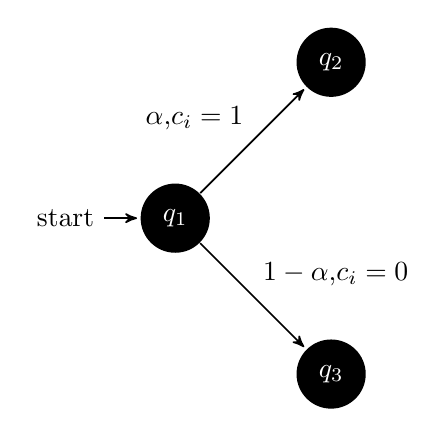
\begin{tikzpicture}[->,>=stealth',shorten >=1pt,auto,node distance=2.8cm,
 semithick]
 \tikzstyle{every state}=[fill=black,draw=none,text=white]
 \node[initial,state] (A)                    {$q_1$};
 \node[state]         (B) [above right of=A] {$q_2$};
 \node[state]         (C) [below right of=A] {$q_3$};
 
 \path (A) edge              node {$\alpha$,$c_i=1$} (B)
 edge              node {$1-\alpha$,$c_i=0$} (C);
 \end{tikzpicture}
 
 Second action is, sending two other players two random values calculated. For a Byzantine player there are four possibilities. In the diagram possibilities for sending different binary values to two remaining players is shown.
 
 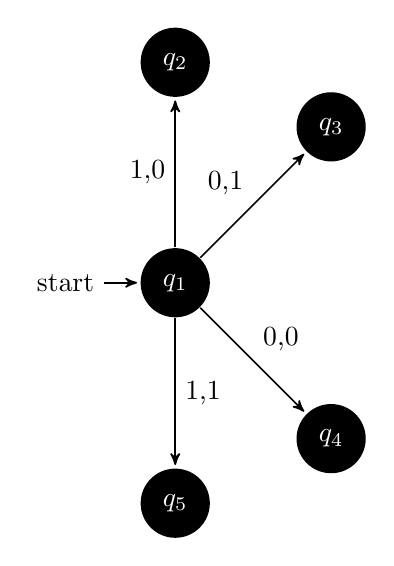
\begin{tikzpicture}[->,>=stealth',shorten >=1pt,auto,node distance=2.8cm,
 semithick]
 \tikzstyle{every state}=[fill=black,draw=none,text=white]
 \node[initial,state] (A)                    {$q_1$};
 \node[state]         (B) [above of =A] {$q_2$};
 \node[state]         (C) [above right of=A] {$q_3$};
 \node[state]         (D) [below right of=A] {$q_4$};
 \node[state]         (E) [below of =A] {$q_5$};
 
 \path (A) edge              node {1,0} (B)
 edge              node {0,1} (C)
 edge              node {0,0} (D)
 edge              node {1,1} (E);
 \end{tikzpicture}
 
 In this example, the set $Z=\{\}$ so that each player is either Altruistic or Rational. The pay-off function is only defined for actions which end in terminal states. For all other actions pay-off is simply $0$. Let the value $\beta_i=1$ $\forall i$ (which is a deviation from the proposed approach) For any infinite length path, the value function would always be a finite value. As a result, discount factor is not essential here. Possible values of the value functions according to these reductions would be an expected utility value under some non-deterministic choice. Then the probabilistic path for maximum utility is same as the path for maximum value in this model.
 Terminal actions are the actions where at least one player learns the secret. In all the other actions, the transition state would be the initial state itself.\\
 The protocol was modelled in PAT  to verify the reaching probabilities of each terminal state. It was verified that the protocol is a Nash equilibrium when $\alpha_i=0.3 \text{ for each }i$.
%We have modelled this mechanism in PAT for $3$ out of $3$ secret sharing case and verified the expected running times, %generated attack traces and verified attack probabilities. In this work they have general utility values for scenarios ui(only $i$ %knows the secret), ui (everyone knows the secret) and ui (no one knows the secret) such that 
%$u_i(only $i$ knows the secret) > u_i (everyone knows the secret)> u_i (no one knows the secret)$. Even though players have %no incentive to cheat and violate the protocol in the long run (when α is chosen carefully). PAT model checker, extended with %Nash equilibrium verifier proves that the protocol is rational. 

\section{EXPERIMENTAL RESULTS}
Experiments are based on the example mechanism presented in section \ref{ssec:ex}. Exact same mechanism is tested for running time and memory performance for different numbers of players and different Byzantine set sizes. In all cases $\epsilon=0.01$ and $\delta=0.005$. Experiments were run in 64-bit x-86 Intel machine having 2.40 GHz processor with 8GB RAM.

\begin{table}[H]
	\centering
	\caption{Experimental Results }
	\label{my-label}
	\resizebox{\columnwidth}{!}{
	\begin{tabular}{|l|l|l|l|l|l|l|l|}
		\hline
		Agents & Jobs & Byzantines & Nash & CPU(sec) & Present State Bits & Action Bits \\ \hline
		3      & 2    & 1          & PASS & 7.8405   &  9                 &  3          \\
		3      & 2    & 2          & PASS & 16.7238  &  9                 &  3          \\
		3      & 2    & 3          & FAIL & 7.6124   &  9                 &  3          \\
		4      & 2    & 1          & PASS & 979.3278 &  12                &  4          \\
		4      & 2    & 2          & FAIL & 1667.687 &  12                &  4          \\
		4      & 2    & 3          & FAIL & 1892517  &  12                &  4          \\ \hline
	\end{tabular}
}
\end{table}
%\section{CASE STUDIES}
To validate our algorithm and implementations, we performed two case studies.

%\input{rabin}
\section{CASE STUDY: ANALYZING A PROBABILISTIC SECRET SHARING SCHEME}

we performed a case study on a probabilistic secret sharing scheme~\cite{HT04} by modelling according to the proposed probabilistic approach in section \ref{ssec:prob_act} with some protocol specific improvements.

\emph{Secret sharing} is a way for a group of users to share a \emph{secret}: the secret is distributed among the group members, such that each member has a \emph{share} of the secret; and the secret can only be reconstructed with a sufficient number of shares. In other words, the secret is kept confidential, even in the presence of a limited number of traitors (compromised members or non-cooperating members who prevent the reconstruction of the secret). This property makes secret sharing an ideal scheme for storing high sensitive informations, such as encryption keys and launch codes. In the parametric form, a $n\mbox{-}m$ ($n\geq m$) secret sharing ensures that it requires at least $m$ honest players to reconstruct the secret within a group of $n$ players. In other words, less than $m$ compromised players together cannot reconstruct the secret; and less than $n-m$ non-cooperating members together cannot stop the honest players to reconstruct of the secret.

The most well-known secret sharing scheme is the Shamir's secret sharing~\cite{Shamir79}. However, the scheme does not work when the players are \emph{rational} -- a player follows the protocol only if it increases his utility. It is shown that a rational player will not share his secret with anyone else. ~\cite{HT04}.  In fact, it is proved that in general, in all practical mechanisms for shared-secret reconstruction with an upper bound on the running time, the best strategy for each rational player is doing nothing~\cite{HT04}. Hence, a randomized mechanism (the probabilistic secret sharing scheme) is proposed to ensure that rational players would reveal their shares to reconstruct the secret, i.e., achieving a Nash-Equilibrium with a constant expected running time. 

The probabilistic scheme is a $3\mbox{-}3$ secret sharing\footnote{A general $n\mbox{-}m$ secret sharing is considered as variations of the basic $3\mbox{-}3$ secret sharing (for details, see~\cite{HT04})}. 
Given the $3$ players, we index each player is indexed with a distinct number in $\{1, 2, 3\}$. We use $i$ to denote one player, then the other two players are $(i+1)\%3$, denoted as $i^+$, and $(i-1)\%3$, denoted as $i^-$. There is an issuer who assign each player a share of secret. Assuming the share cannot be changed; for example, it is signed by the issuer.
The scheme works as follows.
\begin{enumerate}
\item Each player $i$
\begin{itemize}
\item chooses a bit $c_i$ ($c_i$ can only be $1$ or $0$) such that $c_i =1$ with probability $\alpha$ and $c_i = 0$ with probability $1-\alpha$; 
\item chooses a bit $c_{(i,+)}$ ($c_{(i,+)}$ can only be $1$ or $0$) randomly, so that $c_{(i,+)}=1$ with probability $1/2$ and $c_{(i,+)}=0$ with probability $1/2$;
\item calculates $c_{(i,-)}= c_i \xor c_{(i,+)}$. 
\end{itemize}
Then player $i$ sends the bit $c_{(i,+)}$ to player $i^+$ and sends the bit $c_{(i,-)}$ to player $i^-$. This means that the player $i$ receives a bit $c_{(i^+,-)}$ from player $i^+$ and a bit $c_{(i^-,+)}$ from player $i^-$.
\item On receiving $c_{(i^+,-)}$, player $i$ computes $c_{(i^+,-)} \xor c_i$ and sends it to player $i^-$. Correspondingly, $i$ receives $c_{((i^+)^+, -)} \xor c_{i^+}$ from $i^+$. Since there are only $3$ players, player $(i^+)^+$ is the player $i^-$. Hence $c_{((i^+)^+, -)} \xor c_{i^+}=c_{(i^-,-)} \xor c_{i^+}$.
\item When receiving both $c_{(i^-,+)}$ from player $i^-$ (step 1) and receiving $c_{(i^-,-)} \xor c_{i^+}$ from $i^+$ (step 2), $i$ computes $p = c_{(i^-,+)} \xor (c_{(i^-,-)}\xor c_{i^+})\xor c_i$. Note that $ c_{(i^-,+)} \xor (c_{(i^-,-)}\xor c_{i^+})\xor c_i=c_{i^-} \xor c_{i^+}\xor c_i$, i.e., $p=c_1 \xor c_2 \xor c_3$ (It holds for all players).
If $p = c_i = 1$ then player $i$ sends his share to the others.
\item Depending on the value of $p$ and $c_i$, player $i$ decides whether to send his share.
\begin{itemize}
\item If $p=1$, $i$ receives $3$ shares, then he construct the secret.
\item If $p =0$ and $i$ received no secret shares, or if $p =1$ and $i$ received exactly one share (possibly from itself; that is, we allow the case that $i$ did not receive any shares from other players but sent its own), the issuer restarts the protocol. 
\item Otherwise, player $i$ stops the protocol. Because someone must have been cheating. 
\end{itemize}
The intuition behind the last step is as follows: When $p=0$, no one should send his share; and thus $i$ receives no secret share. Otherwise, some one calculated wrong (cheating).
When $p=1$ either $c_i=c_{i^+}=c_{i^-}=1$ or there exists exactly one player chooses $1$, i.e., $c_i=c_{i^+}=0$ and $c_{i^-}=1$, $c_i=c_{i^-}=0$ and $c_{i^+}=1$, or $c_{i^+}=c_{i^-}=0$ and $c_i=1$. 
In the former case, each player can construct the secret. In the later case, $i$ should receive exactly one share. Otherwise, some player calculated wrong (cheating). 
\end{enumerate}

\paragraph{Model}
The above randomized version of the shamir secret sharing scheme can be modelled with the probabilistic extension proposed.\newline

Here, we assume that message channels are secure and sender's authenticity is preserved.
The above protocol is a deterministic protocol where at each step an honest player has to perform a single predefined task(may be probabilistic), depending on the global state he/she is in. This scenario has a unique initial global state. Let's say player $i$'s initial state is $s_{i0}$. The initial global state is is unique here so that, $I=\{(s_{10},s_{20},s_{30}) \}$.
Let's have a look at their Byzantine behaviours starting from the initial state.
 
 \begin{enumerate}
 	\item Player $i$'s probabilistic action to choose $c_i$. $c_i=1$ with probability $\alpha$. 
 	\item choose $c_{i^+}$ with $0.5$ probability.
 	\item send messages to $(i^{+}$ and $i^{-}$. (since the messages are boolean, player has four different actions )
 	\item send 'xor' to player $i^{-}$. (two options - sending correct one or incorrect one)
 	\item send or not send the messages to player $i^-$ and $i^+$. (total four possibilities)
 	\item restart the protocol
 \end{enumerate}
 The above actions sets are activated in different levels. For example, first action set starts from the initial state.
 
 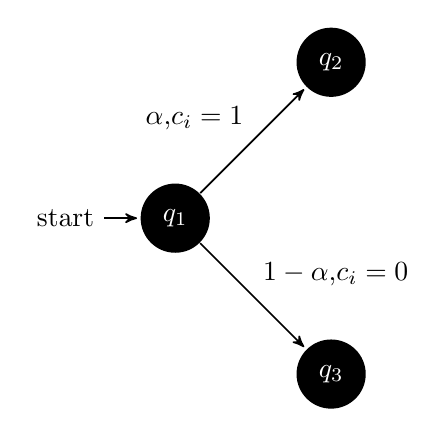
\begin{tikzpicture}[->,>=stealth',shorten >=1pt,auto,node distance=2.8cm,
 semithick]
 \tikzstyle{every state}=[fill=black,draw=none,text=white]
 \node[initial,state] (A)                    {$q_1$};
 \node[state]         (B) [above right of=A] {$q_2$};
 \node[state]         (C) [below right of=A] {$q_3$};
 
 \path (A) edge              node {$\alpha$,$c_i=1$} (B)
 edge              node {$1-\alpha$,$c_i=0$} (C);
 \end{tikzpicture}
 
 Second action is, sending two other players two random values calculated. For a Byzantine player there are four possibilities. In the diagram possibilities for sending different binary values to two remaining players is shown.
 
 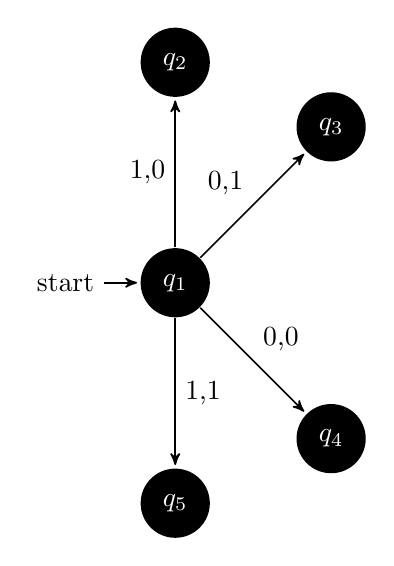
\begin{tikzpicture}[->,>=stealth',shorten >=1pt,auto,node distance=2.8cm,
 semithick]
 \tikzstyle{every state}=[fill=black,draw=none,text=white]
 \node[initial,state] (A)                    {$q_1$};
 \node[state]         (B) [above of =A] {$q_2$};
 \node[state]         (C) [above right of=A] {$q_3$};
 \node[state]         (D) [below right of=A] {$q_4$};
 \node[state]         (E) [below of =A] {$q_5$};
 
 \path (A) edge              node {1,0} (B)
 edge              node {0,1} (C)
 edge              node {0,0} (D)
 edge              node {1,1} (E);
 \end{tikzpicture}
 
 In this example, the set $Z=\{\}$ so that each player is either Altruistic or Rational. The pay-off function is only defined for actions which end in terminal states. For all other actions pay-off is simply $0$. Let the value $\beta_i=1$ $\forall i$ (which is a deviation from the proposed approach) For any infinite length path, the value function would always be a finite value. As a result, discount factor is not essential here. Possible values of the value functions according to these reductions would be an expected utility value under some non-deterministic choice. Then the probabilistic path for maximum utility is same as the path for maximum value in this model.
 Terminal actions are the actions where at least one player learns the secret. In all the other actions, the transition state would be the initial state itself.\\
 The protocol was modelled in PAT  to verify the reaching probabilities of each terminal state. It was verified that the protocol is a Nash equilibrium when $\alpha_i=0.3 \text{ for each }i$.
%We have modelled this mechanism in PAT for $3$ out of $3$ secret sharing case and verified the expected running times, %generated attack traces and verified attack probabilities. In this work they have general utility values for scenarios ui(only $i$ %knows the secret), ui (everyone knows the secret) and ui (no one knows the secret) such that 
%$u_i(only $i$ knows the secret) > u_i (everyone knows the secret)> u_i (no one knows the secret)$. Even though players have %no incentive to cheat and violate the protocol in the long run (when α is chosen carefully). PAT model checker, extended with %Nash equilibrium verifier proves that the protocol is rational. 

\section{CONCLUSIONS AND FUTURE WORK}
We presented a model checking algorithm  to verify Nash Equilibrium in deterministic, probabilistic protocols in finite state concurrent systems. We specify such protocols as probabilistic finite automata and verify $\epsilon-f-Nash$\cite{MMS08} by using the proposed algorithm. We evaluated the applicability of the protocol with a case study about randomized secret sharing protocol\cite{HT04} and presented the experimental results via a continuous task sharing scenario.\newline

As future work, we will support non-deterministic protocols with the presence of probabilistic actions (Markov Decision Processes). We also plan to develop a tool to convert a finite state concurrent system specification to a game with the least involvement of the designer.  
\bibliographystyle{abbrv}
\bibliography{FM}
\appendix

\section{Proofs}

In order to prove the convergence of the value function we should find a function to determine the value difference.\newline
Define $e_i(k)=\beta_i^{k}\frac{M_i}{1-\beta_i}$. 



\begin{lemma}
	\label{lem : conv_vi_path4}
	\begin{enumerate}
		\item $\forall k\in \mathbb{N}, |v_i(\{\pi\})-v_i(\{\pi|_k\})|$ $\le$ $e_i(k)$.	
		\item $\lim_{k\to\infty} v_i(\{\pi\})=v_i(\{\pi|_k\})$
		\end{enumerate}
		\end{lemma}
		
		
		\begin{proof}
			%	Let $\pi''^{a}=<b,\pi'^{a}>$ , $b \in A$\newline
			Consider the absolute difference for $T$-length path tree and fixed $k$-length path tree as follows.
			\begin{enumerate}
				\item 	$|v_i(\{\pi|_T\})-v_i(\{\pi|_k\})| =$\\
				$| E_{\pi^{'a} \in \Pi_{t=0}^{k-1} A_{[n]-Z}}(\Sigma_{t=0}^{k-1} \beta_i^{t}h_{i}(\pi^{s}(t),\pi^{a}(t))) -$\newline
				$ E_{\pi''^{a} \in \Pi_{t=0}^{k-1} A_{[n]-Z} \Pi_{t=k}^{T} A_{[n]-Z}}(\Sigma_{t=0}^{T} \beta_i^{t}h_{i}(\pi''^{s}(t),\pi''^{a}(t)))|$\\
				\newline
				We need to equalize the variable set considered expected value. We just append the variables that do not appear in the expected value function to the considered variable set since it does not make any difference. \newline \newline
				$| E_{\pi''^{a} \in \Pi_{t=0}^{k-1} A_{[n]-Z} \Pi_{t=k}^{T} A_{[n]-Z}}(\Sigma_{t=0}^{k-1} \beta_i^{t}h_{i}(\pi^{s}(t),\pi^{a}(t)))-$\newline
				$ E_{\pi''^{a} \in \Pi_{t=0}^{k-1} A_{[n]-Z} \Pi_{t=k}^{T} A_{[n]-Z}}(\Sigma_{t=0}^{T} \beta_i^{t}h_{i}(\pi''^{s}(t),\pi''^{a}(t)))|$\\
				$ |E_{\pi''^{a} \in \Pi_{t=0}^{k-1} A_{[n]-Z} \Pi_{t=k}^{T} A_{[n]-Z}}(\Sigma_{t=k}^{T} \beta_i^{t}h_{i}(\pi''^{s}(t),\pi''^{a}(t)))|$\\
				$\leq |\Sigma_{t=k}^{T} E_{\pi''^{a} \in \Pi_{t=0}^{k-1} A_{[n]-Z} \Pi_{t=k}^{T} A_{[n]-Z}}( \beta_i^{t}h_{i}(\pi''^{s}(t),\pi''^{a}(t)))| $ (Linearity of Expectation)\\
				$\leq \Sigma_{t=k}^{T}| E_{\pi''^{a} \in \Pi_{t=0}^{k-1} A_{[n]-Z} \Pi_{t=k}^{T} A_{[n]-Z}}( \beta_i^{t}h_{i}(\pi''^{s}(t),\pi''^{a}(t)))| $ (Triangle inequality)\\
				$\le \beta_i^{k}\frac{M_i}{1-\beta_i}$ (By the choice of $M_i$ and $\lim_{T\to\infty}$)\\
				$\leq e_i(k)$
				\item $\lim_{k\to\infty} e_i(k)=0$,\\
				$\lim_{k\to\infty} |v_i(\{\pi\})-v_i(\{\pi|_k\})| = 0$ (by comparison test)\\
				$\lim_{k\to\infty} v_i(\{\pi\})=v_i(\{\pi|_k\})$.
				\end{enumerate}
				\end{proof}
				
				\begin{lemma}
					\label{lem : opt_finite_path5}
					Let $\{ \pi \}$ be a path tree s.t. $v_i(\{\pi\})$ is minimum in $Path(s,Z,i,\{\sigma\})$. Let $\{\{\bar\pi_k \} \}_{k \in \mathbb{N}}$ be a sequence of finite path, s.t. $\forall k$, $v_i(\{\bar\pi_k   \})$ is minimum in $Path_k(s,Z,i,\{\sigma\})$. Then $v_i(\{\pi|_k\})-v_i(\{\bar\pi_k\}) \le 2e_i(k)$
					\end{lemma}\cite{MariPhD}
					
					\begin{lemma}
						\label{lem : opt_finite_strat6}
						$\forall Z \in [n]$, $\forall \text{state s} \in S$ and $\forall strategy$ $sets \{\sigma\}$ we have \\
						$\lim_{k\to\infty} v_i^{k}(Z,s,\{\sigma\}|_k) = v_i(Z,s,\{\sigma\}) $
						\end{lemma}\cite{MariPhD}
						
						\begin{lemma}
							\label{lem : conv_vi7}
							$\forall Z \subseteq [n]$, $\forall \text{states s} \in S$ and $\forall k \in \mathbb{N}$, we have:\\
							$|v_i^{k}(Z,s)-v_i(Z,s)| < 5e_i(k)$
							\end{lemma}\cite{MariPhD}
							
							\begin{lemma}
								\label{lem : conv_ui8}
								$\forall Z \subseteq [n]$, $\forall \text{states s}$ and $\forall k \in \mathbb{N}$, we have: \\
								$|u_i^{k}(Z,s) - u_i(Z,s)| < 5e_i(k)$
								\end{lemma}\cite{MariPhD}
								
								By referring to the above lemmas we can state the following proposition. \\
								
								\begin{proposition}
									\begin{enumerate}
										\item $\lim_{k\to\infty} v_i^{k}(Z,s)=v_i(Z,s)$
										\item $\lim_{k\to\infty} u_i^{k}(Z,s)=u_i(Z,s)$
										\end{enumerate}
										\end{proposition} \cite{MariPhD}
										
										Now we can prove the theorem \ref{thm : correctness}.\\
										By Lemma \ref{lem : conv_vi7} and \ref{lem : conv_ui8} we have, \\
										$\forall Z \in P_\chi([n]-\{i\})$ and $\forall states s \in S$\\
										$|v_i^{k}(Z,s)-v_i(Z,s)| < 5e_i(k)$\\
										$|u_i^{k}(Z,s) - u_i(Z,s)| < 5e_i(k)$\\
										This will imply,\\
										$v_i(Z \cup \{i\},s) \le v_i^{k}(Z \cup \{i\},s) + 5e_i(k)$  By Lemma $ \ref{lem : opt_finite_path5}$\\
										$v_i(Z \cup \{i\},s) \ge v_i^{k}(Z \cup \{i\},s) - 5e_i(k)$  By Lemma $ \ref{lem : opt_finite_strat6}$\\
										$u_i(Z ,s) \le u_i^{k}(Z ,s) + 5e_i(k)$  By Lemma $ \ref{lem : conv_vi7}$\\
										$u_i(Z ,s) \ge u_i^{k}(Z ,s) - 5e_i(k)$  By Lemma $ \ref{lem : conv_ui8}$\\
										\cite{MariPhD}
										Now, we can prove the $3$ statements.\\
										\begin{enumerate}
											\item Using Lemma \ref{lem : opt_finite_path5} and Lemma \ref{lem : conv_ui8},\\
											$v_i(Z \cup \{i\},s) - u_i(Z ,s) \le v_i^{k}(Z \cup \{i\},s) + 5e_i(k) - (u_i^{k}(Z ,s) - 5e_i(k) )$\\
											$=v_i^{k}(Z \cup \{i\},s) - u_i^{k}(Z ,s) + 10e_i(k)  $\\
											$\le \Delta_i(k) + 10e_i(k) $\\
											if $\epsilon \ge \epsilon_2(i,k)$ then $\Delta_i(k) \le \epsilon - 10e_i(k)$\\
											So, $\forall Z \in P_\chi([n]-\{i\})$ and $\forall s \in I$, \\
											$v_i(Z \cup \{i\},s) - u_i(Z ,s) \le \epsilon$\\
											$M$ is $\epsilon - \chi-Nash$.
											\item Similarly, \ref{lem : opt_finite_strat6} and \ref{lem : conv_vi7} can be used to prove\\
											$v_i(Z \cup \{i\},s) - u_i(Z ,s) \ge v_i^{k}(Z \cup \{i\},s) - 5e_i(k) - (u_i^{k}(Z ,s) + 5e_i(k) )$\\
											$=v_i^{k}(Z \cup \{i\},s) - u_i^{k}(Z ,s) - 10e_i(k)  $\\
											if $\epsilon \le \epsilon_1(i,k)$ then $\Delta_i(k) \ge \epsilon + 10e_i(k)$\\
											This implies $\exists Z \in P_\chi([n]-\{i\})$ and $s \in I$ s.t.\\
											$v_i(Z \cup \{i\},s) - u_i(Z ,s) \ge \epsilon$\\
											$M$ is not $\epsilon-\chi-Nash$.
											\item if $\forall i$, $\epsilon_1(i,k_i) < \epsilon$ and for some $j, \epsilon < \epsilon_2(j,k_j)$, \\
											it is not possible to decide whether $M$ is $\epsilon-\chi-Nash$. But, since $\epsilon_2(j,k_j)-\epsilon_1(i,k_i)= 20e_i(k_i)$ and $20e_i(k_i) < \delta$, we have,\\
											$\forall i \in [n]$, $\epsilon + \delta > \epsilon_2(i,k_i)$. According to statement $1$, we have\\
											$(\epsilon + \delta)-\chi-Nash$.
											\end{enumerate}\cite{MariPhD}

\section{Modelling Randomized Secret Sharing according to the specification}

The protocol we model has $3$ players.

States can be numbered based on the stage of the protocol and the number of actions enabled in previous stage. We can identify stages numbered from $0$ to $6$. \newline Define a function size to determine the number of states in a particular stage.

\begin{itemize}
	\item stage $0$ - initial state - size($0$)= $1$
	\item stage $1$ - after choosing $c_i$ - size($1$)= $2$
	\item stage $2$ - after choosing $c_{i,i+1}$ - size($2$)= $2$
	\item stage $3$ - after sending $c_{i,i-1}$ - size($3$)= $2$
	\item stage $4$ - after sending xor - size($4$)= $2$
	\item stage $5$ - after sending $m$ to $i+1$ - size($5$)= $2$
	\item stage $6$ - after sending $m$ to $i-1$ - size($6$)= $2$
\end{itemize}

A state can be represented by a sequence of integers with length denoting the stage it belongs to, 
and each number of the sequence belonging to the chosen action in each of the previous states.
This numbering mechanism is similar of all the players.

$S_1=\{ x \in seq(\{1,2\}) \vert |x| \le 7 \forall i , x_i \le size(i-1)  \}$\newline
$S_2=\{ x \in seq(\{1,2\}) \vert |x| \le 7 \forall i , x_i \le size(i-1)  \}$\newline
$S_3=\{ x \in seq(\{1,2\}) \vert |x| \le 7 \forall i , x_i \le size(i-1)  \}$\newline


\paragraph{Actions}
We have $3$ action sets, $A_1$ , $A_2$ and $A_3$.\newline
$A_1 = \{ c_1,nc_1, c_{12}, nc_{12},  sr_{12}, sr_{13}, sr_{21}, sr_{31}, nsr_{12}, nsr_{13}, nsr_{21}, nsr_{31}, $ \newline $xor_{13},xor_{21}, nxor_{13},nxor_{21},$\newline $ m_{12}, m_{13},m_{21},m_{31},  nm_{12}, nm_{13},nm_{21},nm_{31}, e\}$
\newline
$A_2 = \{ c_2,nc_2, c_{23}, nc_{23},  sr_{23}, sr_{21}, sr_{32}, sr_{12}, nsr_{23}, nsr_{21}, nsr_{32}, nsr_{12}, $ \newline $
xor_{21},xor_{32}, nxor_{21},nxor_{32},$\newline $m_{21}, m_{23},m_{12},m_{32}, nm_{21}, nm_{23},nm_{12},nm_{32},
e\}$
\newline
$A_3 = \{ c_3,nc_3, c_{31}, nc_{31},  sr_{31}, sr_{32}, sr_{23}, sr_{13}, nsr_{31}, nsr_{32}, nsr_{23}, nsr_{13}, $\newline$
xor_{32},xor_{13}, nxor_{32},nxor_{13},$\newline $m_{32}, m_{31},m_{23},m_{13}, nm_{32}, nm_{31},nm_{23},nm_{13},
e\}$

The set of synchronized actions $A^s$ is, \newline
$A^s = \{ sr_{12},sr_{13},sr_{21},sr_{23},sr_{31},sr_{32}, xor_{13}, xor_{21} , xor_{32} $\newline$
nsr_{12},nsr_{13},nsr_{21},nsr_{23},nsr_{31},nsr_{32}, nxor_{13}, nxor_{21} , nxor_{32}
\}$

\paragraph{Local Transition function}
Transitions happens between consecutive stages of the protocol. For a transition to be valid, the sequence corresponding to current and next states should vary by exactly $1$. Sequence corresponding to the current state should be a prefix of the next state.

\paragraph{Local Action Probabilities}

\begin{equation*}
P_1(s_1,a_1)=
\begin{cases}
\alpha &  s_1=I_1 \wedge a_1=c_1  \\
1 - \alpha &  s_1=I_1 \wedge a_1=nc_1  \\
0.5 &  s_1=I_{11} \vee s_1=I_{12}  \wedge a_1=c_{12} \vee a_1=c_{13} \\
1 & otherwise
\end{cases}	
\end{equation*}

\begin{equation*}
P_2(s_2,a_2)=
\begin{cases}
\alpha &  s_2=I_2 \wedge a_2=c_2  \\
1 - \alpha &  s_2=I_2 \wedge a_2=nc_2  \\
0.5 &  s_2=I_{21} \vee s_2=I_{22}  \wedge a_2=c_{21} \vee a_1=c_{23} \\
1 & otherwise
\end{cases}	
\end{equation*}

\begin{equation*}
P_3(s_3,a_3)=
\begin{cases}
\alpha &  s_3=I_3 \wedge a_3=c_3  \\
1 - \alpha &  s_3=I_3 \wedge a_3=nc_3  \\
0.5 &  s_3=I_{31} \vee s_3=I_{32}  \wedge a_3=c_{32} \vee a_1=c_{31} \\
1 & otherwise
\end{cases}	
\end{equation*}


\section{Definitions of Basic Concepts}
Here are some general definitions of the concepts used in the paper. 
\begin{definition}
	concurrency : The property of program, algorithm, or problem decomposability into order-independent or partially-ordered components or units.This means that even if the concurrent units of the program, algorithm, or problem are executed out-of-order or in partial order, the final outcome will remain the same. This allows for parallel execution of the concurrent units, which can significantly improve the overall speed of execution in multi-processor and multi-core systems.
\end{definition}

\begin{definition}
	Protocol : A set of rules that governs the interaction between agents. 
\end{definition}

Difference between automata and finite state machine
\begin{definition}
	Synchronization:
	Process of precisely coordinating or matching two or more activities, devices, or processes in time
\end{definition}

\begin{definition}
	Game Theory : Game theory is the mathematical study of interaction among independent, self-interested agents. 	
\end{definition}

According to the definition of game theory we can define a game.

\begin{definition}
	Game : Well defined set of interactions among independent self-interested agents.
\end{definition}

\begin{definition}
	Game: A game is defined as a decision tree (or more precisely, a dag) in which every edge, called move, has a polarity indicating whether it is played by the program, called Proponent, or by the environment, called Opponent.
\end{definition}

\begin{definition}
	Alternating Game: A play is alternating when Proponent and Opponent alternate strictly - that is, when neither of them plays two moves in a row.
\end{definition}

\begin{definition}
	Concurrent Game:
\end{definition}

\begin{definition}
	A (finite) concurrent game is a \newline
	tuple G=$\langle h,States,Agt,Act,Mov,Tab \rangle$
	, where $States$ is a \newline 
	(finite) set of states,
	$Agt$ is a  (finite) set of players, $Act$ is a  (finite) set of actions, and
	$Mov : States \times Agt \rightarrow 2^{act} \setminus \{\phi\}$ is a mapping indicating the actions available to a given player in a given state; \newline
	$Tab : States \times Act^{Agt} \rightarrow States$ associates  with  a  given  state  and  a  given move of the players the resulting state.
\end{definition} \cite{bouyer2012concurrent}
The above definition refers to a global state set and can be used for perfect information games. In imperfect information games, some global states are indistinguishable. Probability can also be in-cooperated in to the state transition function.  \cite{gripon2009qualitative}

\begin{definition}
	Protocol as a game : A protocol is a set of rules that governs the interaction between agents. When these agents are self-interested, we can model the protocol as a game. 	
\end{definition}



\end{document}
